% Options for packages loaded elsewhere
\PassOptionsToPackage{unicode}{hyperref}
\PassOptionsToPackage{hyphens}{url}
\PassOptionsToPackage{dvipsnames,svgnames,x11names}{xcolor}
%
\documentclass[
  12pt,
  a4paper,
  DIV=11,
  numbers=noendperiod]{scrartcl}

\usepackage{amsmath,amssymb}
\usepackage{iftex}
\ifPDFTeX
  \usepackage[T1]{fontenc}
  \usepackage[utf8]{inputenc}
  \usepackage{textcomp} % provide euro and other symbols
\else % if luatex or xetex
  \usepackage{unicode-math}
  \defaultfontfeatures{Scale=MatchLowercase}
  \defaultfontfeatures[\rmfamily]{Ligatures=TeX,Scale=1}
\fi
\usepackage{lmodern}
\ifPDFTeX\else  
    % xetex/luatex font selection
\fi
% Use upquote if available, for straight quotes in verbatim environments
\IfFileExists{upquote.sty}{\usepackage{upquote}}{}
\IfFileExists{microtype.sty}{% use microtype if available
  \usepackage[]{microtype}
  \UseMicrotypeSet[protrusion]{basicmath} % disable protrusion for tt fonts
}{}
\makeatletter
\@ifundefined{KOMAClassName}{% if non-KOMA class
  \IfFileExists{parskip.sty}{%
    \usepackage{parskip}
  }{% else
    \setlength{\parindent}{0pt}
    \setlength{\parskip}{6pt plus 2pt minus 1pt}}
}{% if KOMA class
  \KOMAoptions{parskip=half}}
\makeatother
\usepackage{xcolor}
\usepackage[top=20mm,left=20mm,heightrounded]{geometry}
\setlength{\emergencystretch}{3em} % prevent overfull lines
\setcounter{secnumdepth}{-\maxdimen} % remove section numbering
% Make \paragraph and \subparagraph free-standing
\ifx\paragraph\undefined\else
  \let\oldparagraph\paragraph
  \renewcommand{\paragraph}[1]{\oldparagraph{#1}\mbox{}}
\fi
\ifx\subparagraph\undefined\else
  \let\oldsubparagraph\subparagraph
  \renewcommand{\subparagraph}[1]{\oldsubparagraph{#1}\mbox{}}
\fi

\usepackage{color}
\usepackage{fancyvrb}
\newcommand{\VerbBar}{|}
\newcommand{\VERB}{\Verb[commandchars=\\\{\}]}
\DefineVerbatimEnvironment{Highlighting}{Verbatim}{commandchars=\\\{\}}
% Add ',fontsize=\small' for more characters per line
\usepackage{framed}
\definecolor{shadecolor}{RGB}{241,243,245}
\newenvironment{Shaded}{\begin{snugshade}}{\end{snugshade}}
\newcommand{\AlertTok}[1]{\textcolor[rgb]{0.68,0.00,0.00}{#1}}
\newcommand{\AnnotationTok}[1]{\textcolor[rgb]{0.37,0.37,0.37}{#1}}
\newcommand{\AttributeTok}[1]{\textcolor[rgb]{0.40,0.45,0.13}{#1}}
\newcommand{\BaseNTok}[1]{\textcolor[rgb]{0.68,0.00,0.00}{#1}}
\newcommand{\BuiltInTok}[1]{\textcolor[rgb]{0.00,0.23,0.31}{#1}}
\newcommand{\CharTok}[1]{\textcolor[rgb]{0.13,0.47,0.30}{#1}}
\newcommand{\CommentTok}[1]{\textcolor[rgb]{0.37,0.37,0.37}{#1}}
\newcommand{\CommentVarTok}[1]{\textcolor[rgb]{0.37,0.37,0.37}{\textit{#1}}}
\newcommand{\ConstantTok}[1]{\textcolor[rgb]{0.56,0.35,0.01}{#1}}
\newcommand{\ControlFlowTok}[1]{\textcolor[rgb]{0.00,0.23,0.31}{#1}}
\newcommand{\DataTypeTok}[1]{\textcolor[rgb]{0.68,0.00,0.00}{#1}}
\newcommand{\DecValTok}[1]{\textcolor[rgb]{0.68,0.00,0.00}{#1}}
\newcommand{\DocumentationTok}[1]{\textcolor[rgb]{0.37,0.37,0.37}{\textit{#1}}}
\newcommand{\ErrorTok}[1]{\textcolor[rgb]{0.68,0.00,0.00}{#1}}
\newcommand{\ExtensionTok}[1]{\textcolor[rgb]{0.00,0.23,0.31}{#1}}
\newcommand{\FloatTok}[1]{\textcolor[rgb]{0.68,0.00,0.00}{#1}}
\newcommand{\FunctionTok}[1]{\textcolor[rgb]{0.28,0.35,0.67}{#1}}
\newcommand{\ImportTok}[1]{\textcolor[rgb]{0.00,0.46,0.62}{#1}}
\newcommand{\InformationTok}[1]{\textcolor[rgb]{0.37,0.37,0.37}{#1}}
\newcommand{\KeywordTok}[1]{\textcolor[rgb]{0.00,0.23,0.31}{#1}}
\newcommand{\NormalTok}[1]{\textcolor[rgb]{0.00,0.23,0.31}{#1}}
\newcommand{\OperatorTok}[1]{\textcolor[rgb]{0.37,0.37,0.37}{#1}}
\newcommand{\OtherTok}[1]{\textcolor[rgb]{0.00,0.23,0.31}{#1}}
\newcommand{\PreprocessorTok}[1]{\textcolor[rgb]{0.68,0.00,0.00}{#1}}
\newcommand{\RegionMarkerTok}[1]{\textcolor[rgb]{0.00,0.23,0.31}{#1}}
\newcommand{\SpecialCharTok}[1]{\textcolor[rgb]{0.37,0.37,0.37}{#1}}
\newcommand{\SpecialStringTok}[1]{\textcolor[rgb]{0.13,0.47,0.30}{#1}}
\newcommand{\StringTok}[1]{\textcolor[rgb]{0.13,0.47,0.30}{#1}}
\newcommand{\VariableTok}[1]{\textcolor[rgb]{0.07,0.07,0.07}{#1}}
\newcommand{\VerbatimStringTok}[1]{\textcolor[rgb]{0.13,0.47,0.30}{#1}}
\newcommand{\WarningTok}[1]{\textcolor[rgb]{0.37,0.37,0.37}{\textit{#1}}}

\providecommand{\tightlist}{%
  \setlength{\itemsep}{0pt}\setlength{\parskip}{0pt}}\usepackage{longtable,booktabs,array}
\usepackage{calc} % for calculating minipage widths
% Correct order of tables after \paragraph or \subparagraph
\usepackage{etoolbox}
\makeatletter
\patchcmd\longtable{\par}{\if@noskipsec\mbox{}\fi\par}{}{}
\makeatother
% Allow footnotes in longtable head/foot
\IfFileExists{footnotehyper.sty}{\usepackage{footnotehyper}}{\usepackage{footnote}}
\makesavenoteenv{longtable}
\usepackage{graphicx}
\makeatletter
\def\maxwidth{\ifdim\Gin@nat@width>\linewidth\linewidth\else\Gin@nat@width\fi}
\def\maxheight{\ifdim\Gin@nat@height>\textheight\textheight\else\Gin@nat@height\fi}
\makeatother
% Scale images if necessary, so that they will not overflow the page
% margins by default, and it is still possible to overwrite the defaults
% using explicit options in \includegraphics[width, height, ...]{}
\setkeys{Gin}{width=\maxwidth,height=\maxheight,keepaspectratio}
% Set default figure placement to htbp
\makeatletter
\def\fps@figure{htbp}
\makeatother
% definitions for citeproc citations
\NewDocumentCommand\citeproctext{}{}
\NewDocumentCommand\citeproc{mm}{%
  \begingroup\def\citeproctext{#2}\cite{#1}\endgroup}
\makeatletter
 % allow citations to break across lines
 \let\@cite@ofmt\@firstofone
 % avoid brackets around text for \cite:
 \def\@biblabel#1{}
 \def\@cite#1#2{{#1\if@tempswa , #2\fi}}
\makeatother
\newlength{\cslhangindent}
\setlength{\cslhangindent}{1.5em}
\newlength{\csllabelwidth}
\setlength{\csllabelwidth}{3em}
\newenvironment{CSLReferences}[2] % #1 hanging-indent, #2 entry-spacing
 {\begin{list}{}{%
  \setlength{\itemindent}{0pt}
  \setlength{\leftmargin}{0pt}
  \setlength{\parsep}{0pt}
  % turn on hanging indent if param 1 is 1
  \ifodd #1
   \setlength{\leftmargin}{\cslhangindent}
   \setlength{\itemindent}{-1\cslhangindent}
  \fi
  % set entry spacing
  \setlength{\itemsep}{#2\baselineskip}}}
 {\end{list}}
\usepackage{calc}
\newcommand{\CSLBlock}[1]{\hfill\break\parbox[t]{\linewidth}{\strut\ignorespaces#1\strut}}
\newcommand{\CSLLeftMargin}[1]{\parbox[t]{\csllabelwidth}{\strut#1\strut}}
\newcommand{\CSLRightInline}[1]{\parbox[t]{\linewidth - \csllabelwidth}{\strut#1\strut}}
\newcommand{\CSLIndent}[1]{\hspace{\cslhangindent}#1}

\KOMAoption{captions}{tableheading}
\usepackage{wrapfig}
\usepackage{subcaption}
\usepackage{amsmath}
\usepackage{cancel}
\usepackage{hyperref}
\usepackage{tikz}
\usepackage{tabularx}
\usepackage{colortbl}
\usepackage{xcolor}
\renewcommand{\maketitle}{}
\definecolor{winered}{RGB}{164,40,32}
\definecolor{wesgrey}{RGB}{137,157,164}
\usepackage{fancyhdr}
\pagestyle{fancy}
\fancyhf{}
\fancyhead[L]{\rightmark}
\fancyhead[R]{\thepage}
\fancyfoot[C]{\thepage}
\makeatletter
\@ifpackageloaded{caption}{}{\usepackage{caption}}
\AtBeginDocument{%
\ifdefined\contentsname
  \renewcommand*\contentsname{Table of contents}
\else
  \newcommand\contentsname{Table of contents}
\fi
\ifdefined\listfigurename
  \renewcommand*\listfigurename{Figurliste}
\else
  \newcommand\listfigurename{Figurliste}
\fi
\ifdefined\listtablename
  \renewcommand*\listtablename{Tabelliste}
\else
  \newcommand\listtablename{Tabelliste}
\fi
\ifdefined\figurename
  \renewcommand*\figurename{Figur}
\else
  \newcommand\figurename{Figur}
\fi
\ifdefined\tablename
  \renewcommand*\tablename{Tabell}
\else
  \newcommand\tablename{Tabell}
\fi
}
\@ifpackageloaded{float}{}{\usepackage{float}}
\floatstyle{ruled}
\@ifundefined{c@chapter}{\newfloat{codelisting}{h}{lop}}{\newfloat{codelisting}{h}{lop}[chapter]}
\floatname{codelisting}{Listing}
\newcommand*\listoflistings{\listof{codelisting}{List of Listings}}
\makeatother
\makeatletter
\makeatother
\makeatletter
\@ifpackageloaded{caption}{}{\usepackage{caption}}
\@ifpackageloaded{subcaption}{}{\usepackage{subcaption}}
\makeatother
\ifLuaTeX
  \usepackage{selnolig}  % disable illegal ligatures
\fi
\usepackage{bookmark}

\IfFileExists{xurl.sty}{\usepackage{xurl}}{} % add URL line breaks if available
\urlstyle{same} % disable monospaced font for URLs
\hypersetup{
  colorlinks=true,
  linkcolor={blue},
  filecolor={Maroon},
  citecolor={Blue},
  urlcolor={Blue},
  pdfcreator={LaTeX via pandoc}}

\author{}
\date{}

\begin{document}


\newgeometry{left=0cm, right=0cm, top=0cm, bottom=0cm}
\vspace*{0.5cm} 
\hspace*{1.5cm}
\includegraphics[width=10cm]{dokumentobjekter/texstuff/UiT_Logo_Bok_Bla_RGB.png} 


\begin{flushleft}
    \vspace*{0.5cm}
    \hspace*{2.5cm}{\color{black}\fontsize{11}{13.2}\selectfont Handelshøgskolen ved UiT \\[0.2em]
    \hspace*{2.5cm}\color{black}\fontsize{8}{13.2}\selectfont Fakultet for biovitenskap, fiskeri og økonomi \\[0.2em]
    \hspace*{2.5cm}\large{\color{black}\textbf{Mappeoppgave 2}}  \\[0.5em]
    \hspace*{2.5cm}\color{black}\fontsize{12}{14.4}\selectfont Næringsøkonomi og konkurransestrategi\\[0.5em]
\hspace*{2.5cm}\color{black}\fontsize{11}{13.2}\selectfont Kandidatnummer: 30 \\[0.5em]
    \hspace*{2.5cm}\color{black}\fontsize{11}{13.2}\selectfont SOK-2030, Vår 2024 \\[0.5em]
    \hspace*{2.0cm}
    \par}
\end{flushleft} 



\begin{tikzpicture}[remember picture, overlay]
    \node[anchor=south west, inner sep=0] at (current page.south west) {
\includegraphics[width=\paperwidth]{dokumentobjekter/texstuff/forside_bilde.png}};
\end{tikzpicture}


\newgeometry{left=20mm, right=20mm, top=20mm, bottom=20mm}




\thispagestyle{plain}
\begin{center}
    \Large
    \textbf{Sammendrag}
\end{center}

Del opp og strukturer oppgaven bedre.

Forklar bedre og bruk pensum mer på begrunnelse av modeller. 

Lag paier for å illustrere bedre.

Lag en tabell som viser hva og hvilke variabler som er definert i oppgaven.

Lag en tabell som viser profitt med stackelberg og cournot modell i oppgave 1.

Avslutningsvis lag to tabeller som viser profitter til bedriftene før og etter fusjon i oppgave 2 med de forskjellige modellene.

Konklusjon og så få chatgpt til å skrive sammendraget.


\newpage
\hypersetup{linkcolor=black}
\renewcommand{\contentsname}{Innholdsfortegnelse}
\renewcommand*{\figureautorefname}{Figur}
\renewcommand*{\tableautorefname}{Tabell}
\tableofcontents
\newpage
\listoffigures
\listoftables
\hypersetup{linkcolor=blue}
\newpage

\section{Oppslagsverk av variabler}\label{oppslagsverk-av-variabler}

\begin{table}[h]
\centering
\begin{tabular}{|c|c|}
\hline
\rowcolor{winered}
Variabel & Beskrivelse \\ \hline
\rowcolor{wesgrey}
$Q$ & Kvantum \\ \hline
\rowcolor{wesgrey}
$Q{_i^*}$ & Optimalt kvantum for gitt bedrift \\ \hline
\rowcolor{wesgrey}
$P$ & Pris  \\ \hline
\rowcolor{wesgrey}
$P^*$ & Optimal pris \\ \hline
\rowcolor{wesgrey}
$a$ & Maksimal betalingsvillighet \\ \hline
\rowcolor{wesgrey}
$b$ & Koeffisient for prisfølsomhet \\ \hline
\rowcolor{wesgrey}
$c_i$ & Marginale kostnader for gitt bedrift \\ \hline
\rowcolor{wesgrey}
$f_k$ & Faste kostnader for bedrifter \\ \hline
\rowcolor{wesgrey}
$\pi_i$ & Profittfunksjonen for gitt bedrift \\ \hline
\end{tabular}
\caption{Oppslagsverk av variabler}
\label{tab:variabler}
\end{table}

Merk: det er mulighet for notasjonsfeil i \autoref{tab:variabler} mot
hva som er skrevet videre i oppgaven.

\section{Oppgave 1 (30\%)}\label{oppgave-1-30}

Hva blir optimal tilpasning i dette markedet når Olivita kan gjøre sine
strategiske valg før konkurrenten, Dr Choice AS, gjør sitt valg?

\subsection{Valg av modell}\label{valg-av-modell}

Godene vi ser på er substitutter (de er like) hvor Olivita har vært
lengst i markedet og dermed er lederbedriften. Derfor blir
stackelberg-modellen brukt, hvis den ene bedriften (lederbedriften) øker
sin produksjon vil den andre bedriften sin produksjon minke, noe som
gjør det til kvantumkonkurranse.

Stackelberg-modellen er en sekvensiell modell hvor kvantum er
bedriftenes handlingsvariabler i motsetning til bertrand hvor bedriftene
konkurrerer om pris. Lederbedriften Olivita, tar sine beslutninger først
og bestemmer hvor mye som produseres som maksimerer deres egen profitt
basert på at følgerbedriften Dr Choice vil tilpasse seg sekvensielt med
sitt eget kvantum som en reaksjon på Olivita sitt valg av kvantum.

\subsection{Optimal tilpasning ved
stackelberg}\label{optimal-tilpasning-ved-stackelberg}

Ved å bruke en stackelberg modell kan vi finne optimal tilpasning i
markedet.

Den inverse etterspørselen i markedet er gitt ved \(P = a−b(Q_O+Q_C)\)
hvor \(Q_O\) er antall solgte flasker med Olivita, \(Q_C\) er antall
solgte flasker Easy Choice Omega-3 og \(P\) er pris per flaske av
Omega-3 produktene. I produksjon av Omega-3 produktene vil begge
bedriftene ha konstante marginalkostnader \(c\) på kr 50 per produsert
flaske. Faste kostnader \(f_k\) for begge bedriftene er på 3 millioner
kroner. \(a = 990\) og \(b = \frac{1}{60}\) og da blir den inverse
etterspørselen \(P = 990−\frac{1}{60}(Q_O+Q_C)\).

Siden begge bedrifter har samme faste kostnader og marginale kostnader,
kan vi bruke en felles profittfunksjon for begge bedriftene.
Profittfunksjonen er gitt ved:

\[\pi = Q_O(a-b(Q_C+Q_O)-c) \tag{1}\]

Tar så og deriverer profittfunksjonen mhp \(Q_C\):

\[\frac{\partial \pi}{\partial Q_C} = a -b Q_C - b(Q_O+Q_C) -c \tag{2}\]
løser for kvantum og setter den deriverte lik 0 for å finne
reaksjonfunksjonen til Dr Choice AS

\[ Q_C = \frac{a-b Q_O -c}{2b} \tag{3}\]

Setter så reaksjonsfunksjonen til Dr Choice inn i profittfunksjonen til
Olivita og deriveres mhp \(Q_O\) og forenkles (ser egentlig mye verre
ut):

\[\frac{\partial \pi}{\partial Q_O} = \frac{a}{2}-bQ_O - \frac{c}{2} \tag{4}\]

Ved å løse for \(Q_O\) får vi optimalt kvantum for lederbedriften
(Olivita), og substituerer inn tallverdier:

\[Q{_O^*} = \frac{a-c}{2b} = \frac{(990 - 50)}{(2 \cdot \frac{1}{60})}  = 28200 \tag{5}\]
Optimalt kvantum for lederbedriften (Olivita) er 28200 flasker.

Og for å finne ut optimalt kvantum for følgerbedriften (Dr Choice)
setter vi inn \(Q{_O^*}\) i reaksjonsfunksjonen til Dr Choice:

\[Q{_C^*} = \frac{a-c}{4b} = \frac{(990 - 50)}{(4 \cdot \frac{1}{60})} = 14100 \tag{6}\]
Hvor optimalt kvantum for følgerbedriften (Dr Choice) blir 14100
flasker.

Videre for å finne optimal pris i sluttmarkedet setter vi inn optimal
\(Q{_O^*}\) og \(Q{_C^*}\) i den inverse etterspørselen:

\[P^* = a - b(Q{_O^*}+Q{_C^*}) = 990 - \frac{1}{60}(28200+14100) = 990 - 705 = 285 \tag{7}\]
Den optimale prisen i sluttmarkedet blir 285 kr per flaske.

Så finner vi profitten til lederbedriften Olivita med å gange optimal
pris med optimalt kvantum \(Q{_O^*}\) og trekker fra marginal kostnader
\(c\) og faste kostnader \(f_k\):

\[ \pi_O = \frac{(a-c)^2}{8b} - f_k =  \frac{(990-50)^2}{(8 \cdot \frac{1}{60})} - 3000000 = 3627000 \tag{8}\]
Profitten til Olivita AS blir å være 3.627.000 kroner.

\clearpage

Til slutt for å finne profitten til følgerbedriften (Dr Choice) så
repeterer vi forrige prosesss bare at vi ganger med optimalt kvantum for
Dr Choice \(Q{_C^*}\):

\[\pi_C = \frac{(a-c)^2}{16b} - f_k =  \frac{(990-50)^2}{(16 \cdot \frac{1}{60})} - 3000000 = 313500 \tag{9}\]
Og finner at profitten til Dr Choice AS blir å være 313.500 kroner.

Den optimale tilpasningen blir 28200 kvantum solgt for Olivita mens Dr
Choice vil tilpasse seg med halvparten av kvantumet på 14100 flasker.

Totalt kvantum blir 42.300 kvantum solgt for begge bedriftene til en
markedspris på 285 kroner per flaske.

Vil det være en fordel for Olivita å ha mulighet til å gjøre sine valg
før konkurrenten gjør sitt valg?

\subsection{Stackelberg ovenfor
cournot}\label{stackelberg-ovenfor-cournot}

For å finne ut om det vil være en fordel for Olivita å ha mulighet til å
gjøre sine valg før Dr Choice, så tar jeg å regner på en cournot modell
for symmetriske bedrifter siden begge bedriftene har samme
marginalkostnader.

Starter likt som med stackelberg og bruker samme etterspørsel og
profittfunksjoner:

\[P = a - b(Q_O+Q_C) \tag{10}\]

\[\pi = Q_O(a-b(Q_C+Q_O)-c) \tag{11}\] Videre så deriverer jeg
profittfunksjonene mhp \(Q_O\) og \(Q_C\):

\[\frac{\partial \pi}{\partial Q_O} = a -b Q_O - b(Q_O+Q_C) -c \tag{12}\]
\[\frac{\partial \pi}{\partial Q_C} = a -b Q_C - b(Q_O+Q_C) -c \tag{13}\]

Og løser for \(Q_O\) og \(Q_C\):

\[Q{_O^*} = \frac{a-c}{3b} = \frac{(990-50)}{(3 \cdot \frac{1}{60})} = 18800 \tag{14}\]

\[Q{_C^*} = \frac{a-c}{3b} \frac{(990-50)}{(3 \cdot \frac{1}{60})} = 18800 \tag{15}\]

Setter så inn \(Q{_O^*}\) og \(Q{_C^*}\) i etterspørselen for å finne
optimal pris i sluttmarkedet:

\[P^* = a - b(Q{_O^*}+Q{_C^*}) = 990 - \frac{1}{60}(18800+18800) = 990 - 626.666 = 363.33 \tag{16}\]

\begin{wrapfigure}{r}{0.5\textwidth}
  \centering
  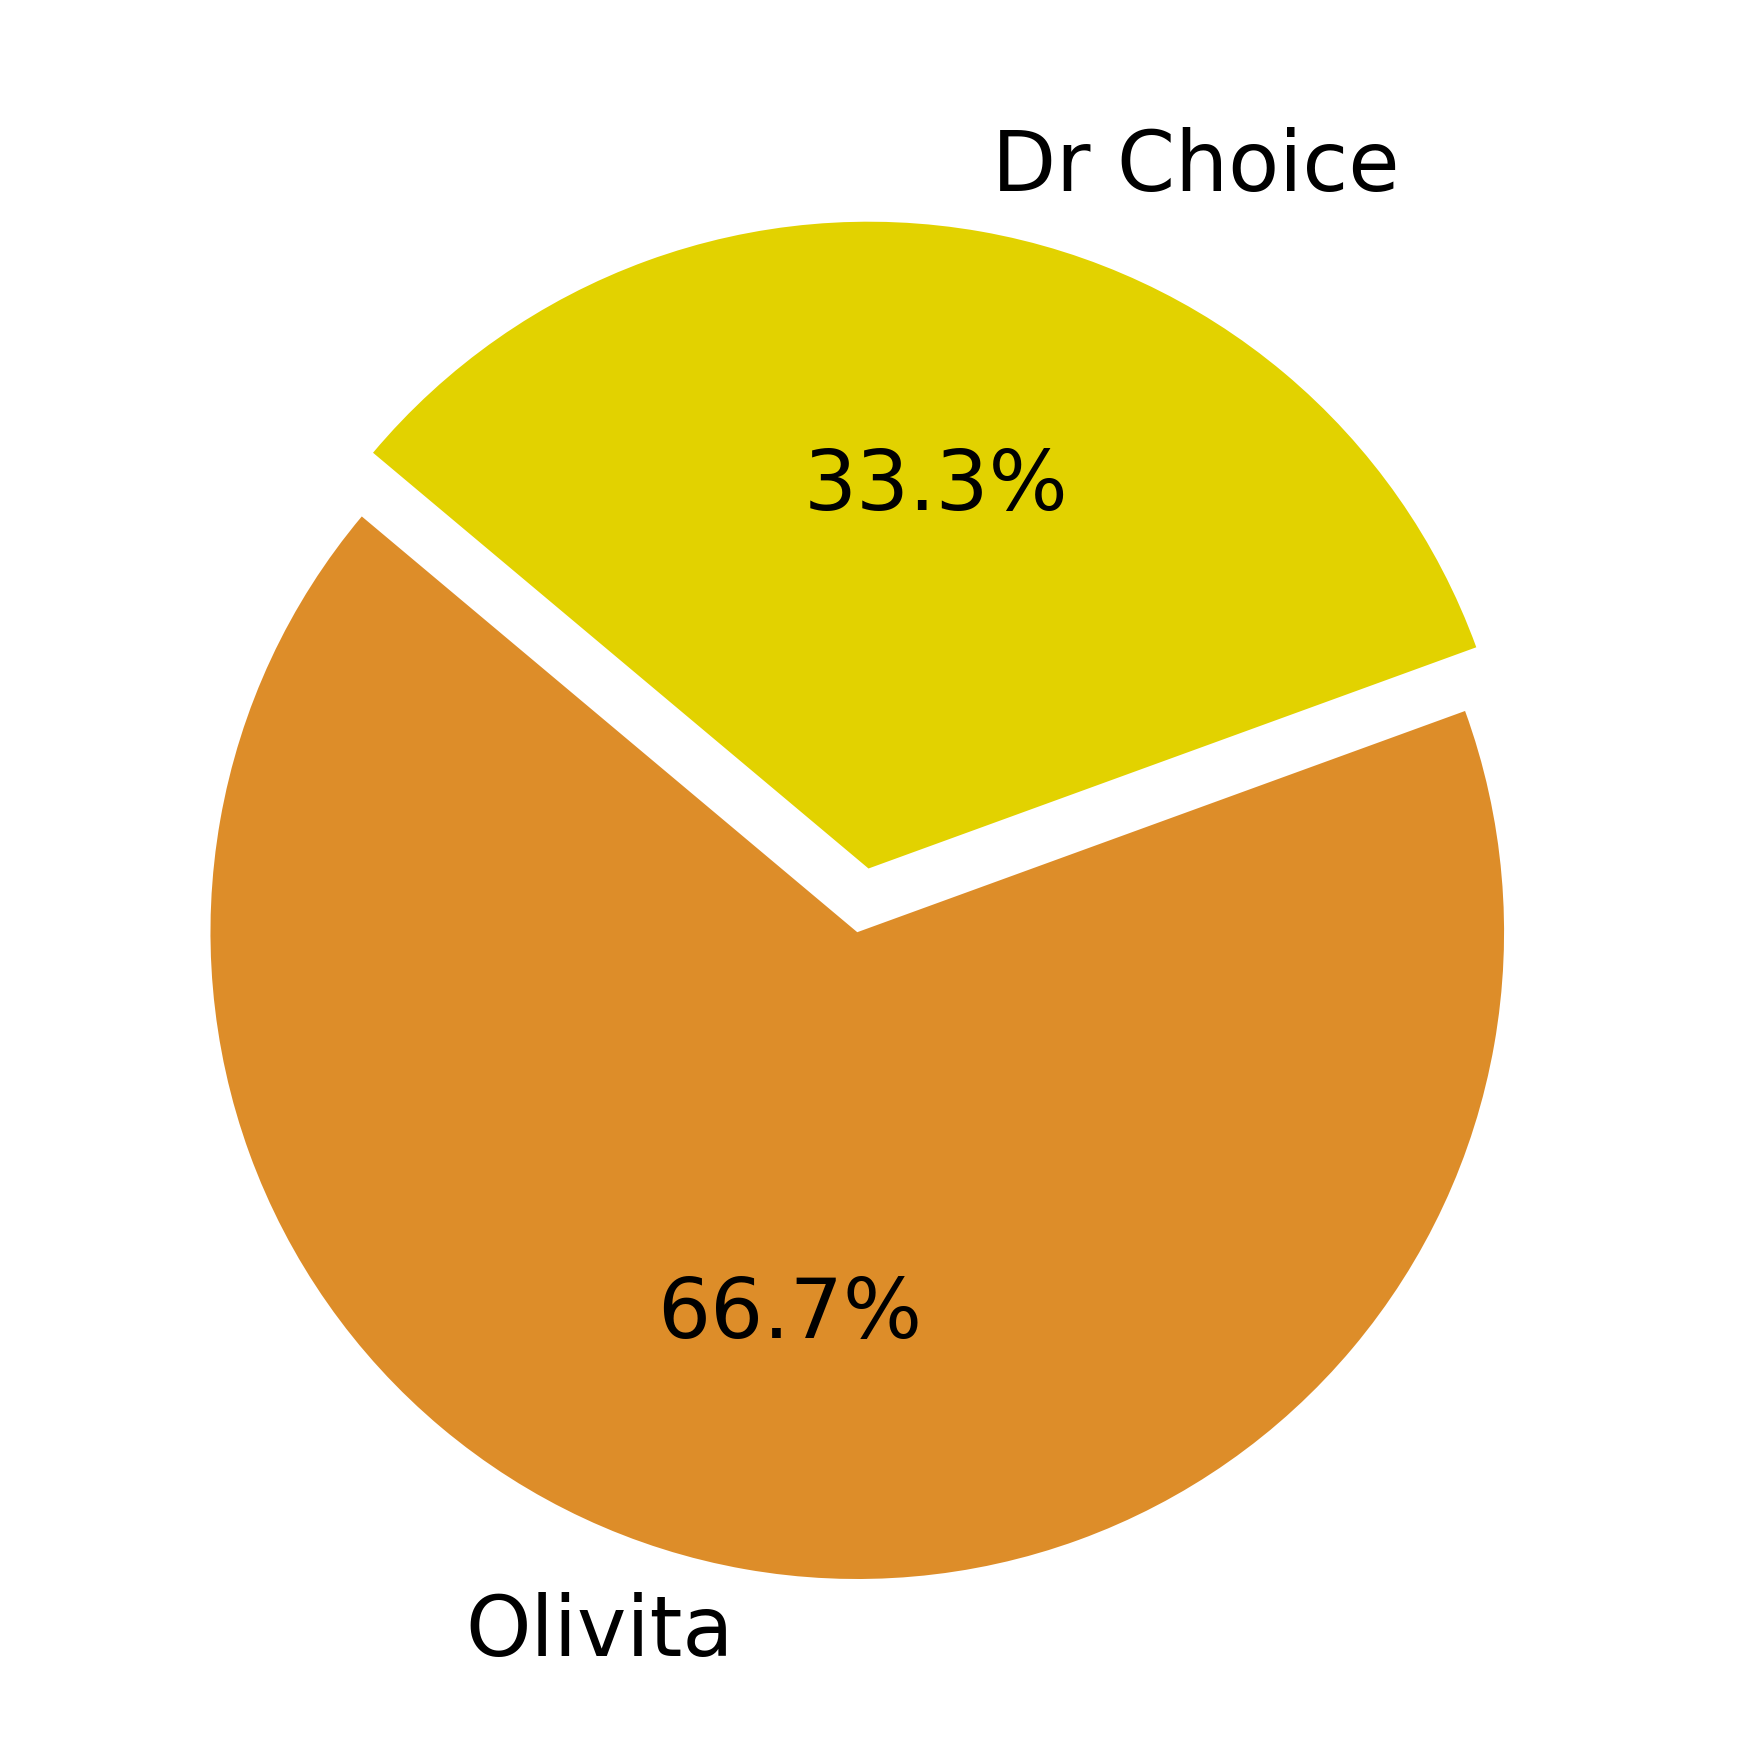
\includegraphics[width=0.5\textwidth]{dokumentobjekter/figurer/stackelberg_olivita_dr_choice.png}
  \captionof{figure}{Stackelberg modell for Olivita og Dr Choice}
  \label{fig:stackel_olivita_dr_choice}
  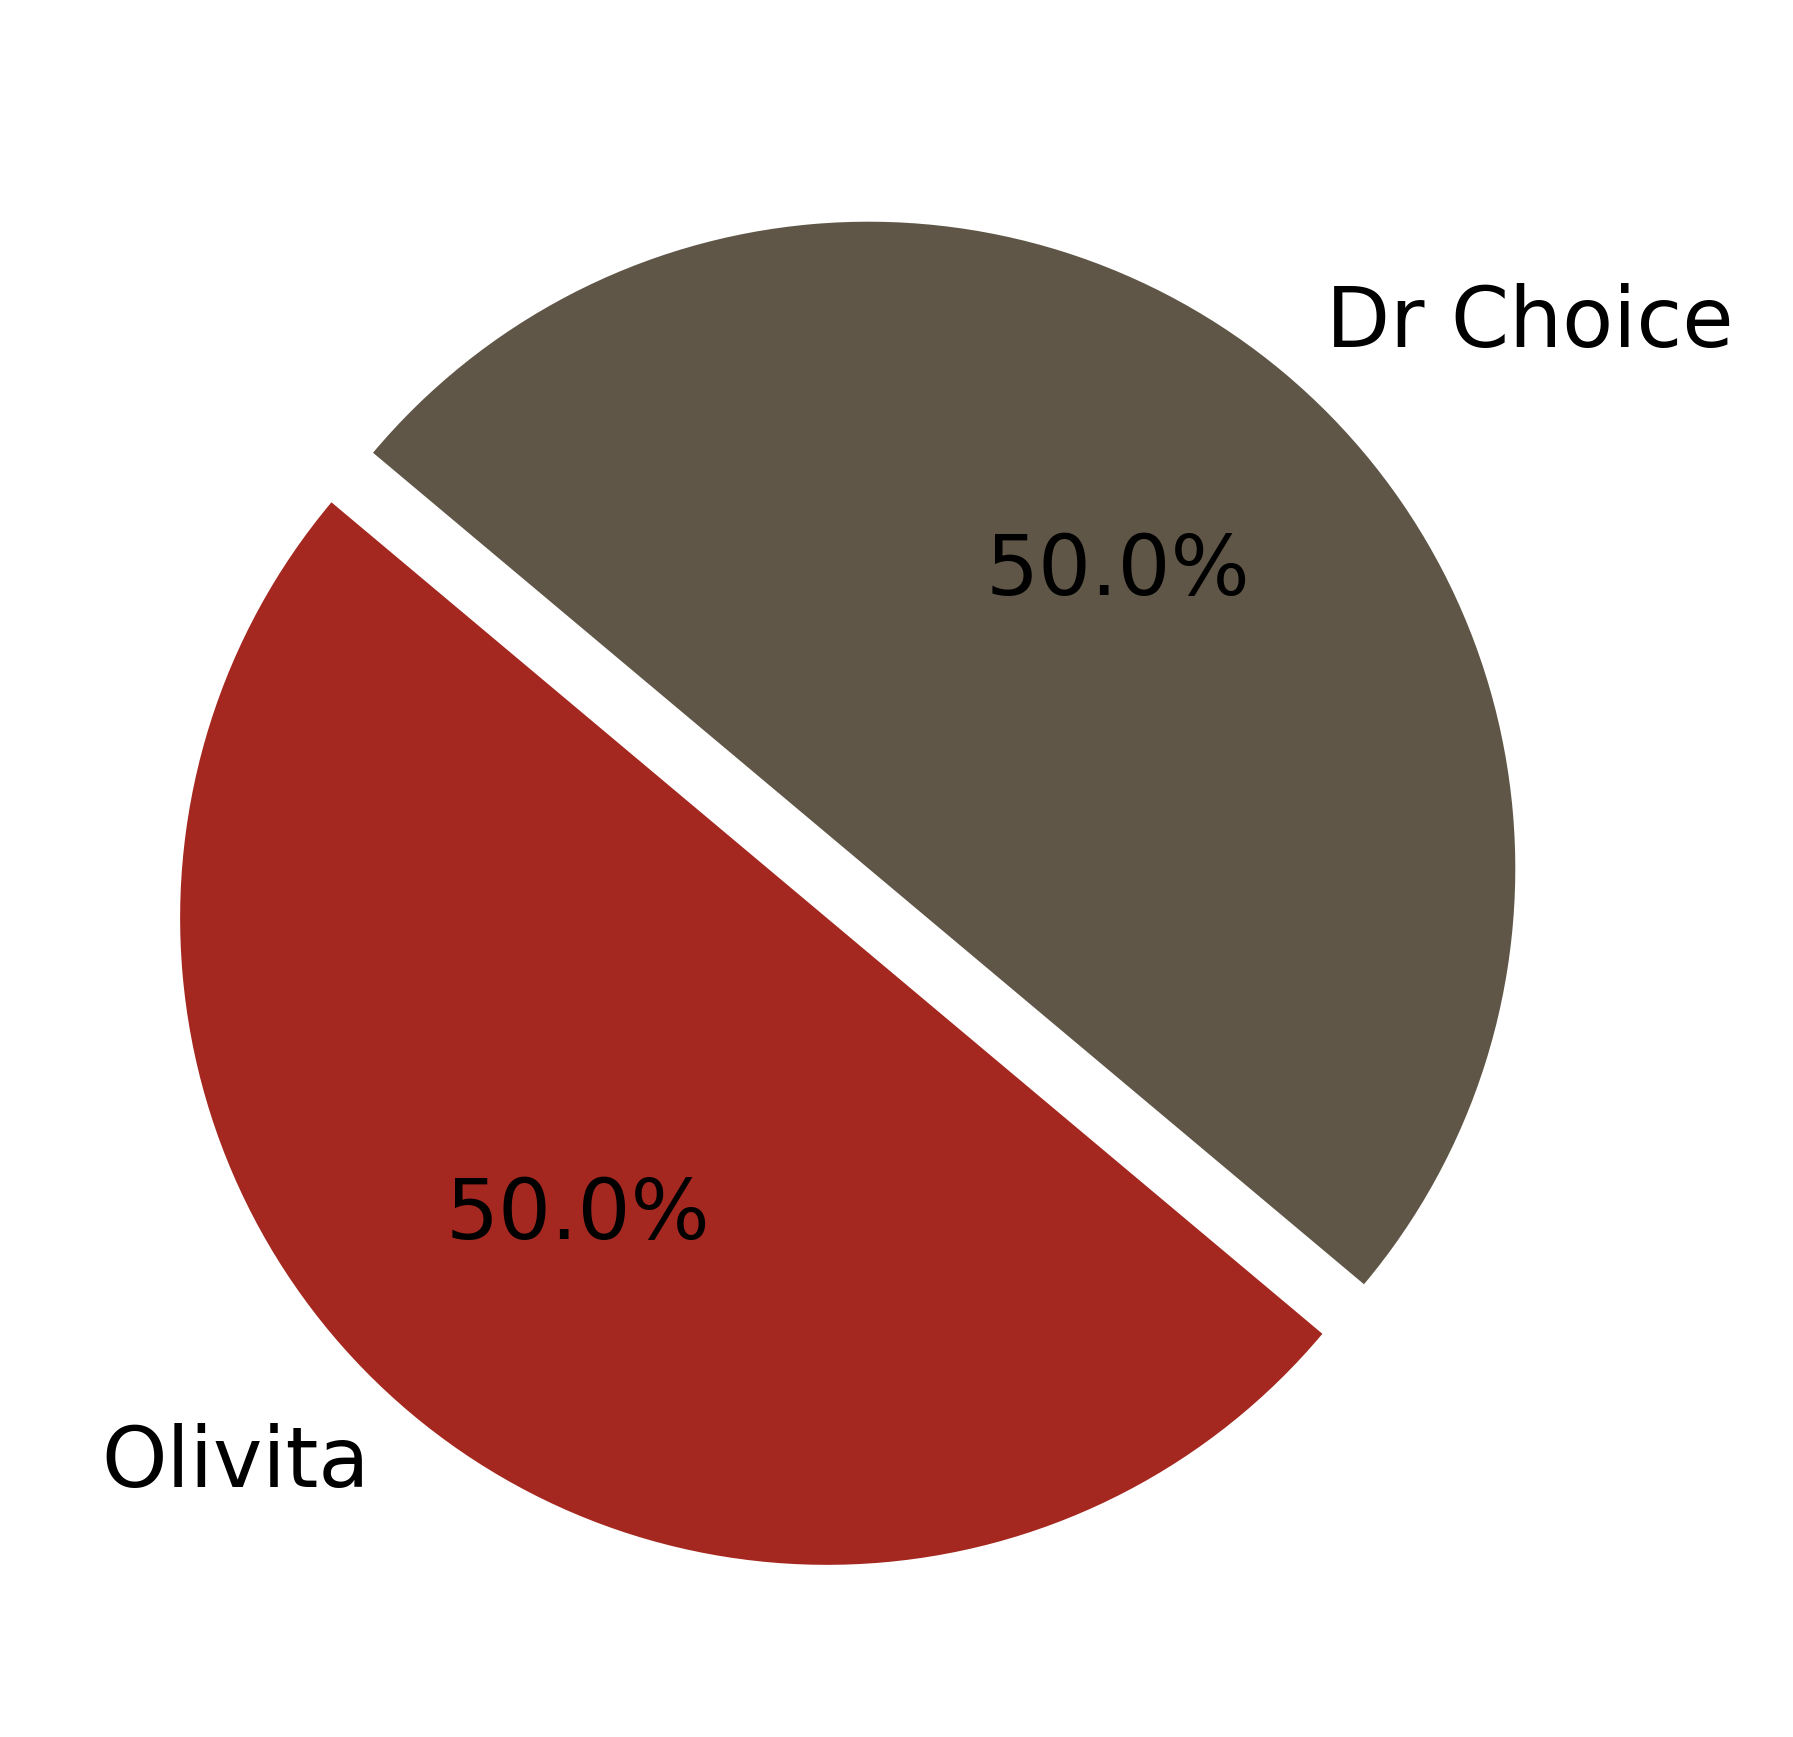
\includegraphics[width=0.5\textwidth]{dokumentobjekter/figurer/cournot_olivita_dr_choice.png}
  \captionof{figure}{Cournot modell for Olivita og Dr Choice}
  \label{fig:cournot_olivita_dr_choice}
  \vspace{-1cm}
\end{wrapfigure}

Fra et samfunnsøkonomisk perspektiv så er det best for samfunnet at
lederbedriften setter prisen først, siden det vil være større kvantum
produsert under stackelberg hvis man ser på
\autoref{table:stackel_cournot} og prisen blir lavere per enhet. Dette
vil føre til at flere kunder vil kjøpe produktet og det vil være en
velferdsgevinst for samfunnet ovenfor cournot. I dette tilfellet blir
totalt kvantum produsert under cournot noe lavere på 37.600, og prisen
per enhet noe dyrere på 363.33 kroner.

Lederbedriften Olivita vil også tjene mer på sekvensielt valg under
stackelberg enn cournot, siden lederbedriften kan sette kvantum
produsert først og følgerbedriften vil tilpasse seg. Dette vil føre til
at lederbedriften vil tjene mer enn følgerbedriften siden de konkurrerer
om kvantum solgt.

Totalt vil lederbedriften tjene 3.627.000 kroner under stackelberg og
\((P^* -c) \cdot Q{_O^*} -f_k =(363 -50) \cdot18800 - 3000000 = 2890666\)
kroner under cournot. Derfor vil det være en fordel for Olivita å ha
mulighet til å gjøre sine valg før Dr Choice gjør sitt valg.

I \autoref{fig:stackel_olivita_dr_choice} kan vi se hvor stor andel av
kvantum produsert hver bedrift får under stackelberg sin modell.
Lederbedriften får \(\frac{2}{3}\) av kaken med 28.200 kvantum produsert
mens følgerbedriften får \(\frac{1}{3}\) av kaken med 14100 enheter
produsert.

I \autoref{fig:cournot_olivita_dr_choice} kan vi se hvor stor andel av
kvantum produsert hver bedrift får under cournot sin modell. Begge
bedriftene får lik andel av kaken med 18.800 kvantum produsert hver.

\begin{wraptable}{r}{8cm}
\centering
\begin{tabular}{|c|c|c|}
\hline
\rowcolor{winered}
 & Stackelberg & Cournot \\ \hline
 \rowcolor{wesgrey}
$Q{_O^*}$ & 28200 & 18800 \\ \hline
 \rowcolor{wesgrey}
$Q{_C^*}$ & 14100 & 18800 \\ \hline
 \rowcolor{wesgrey}
$P^*$ & 285 & 363.33 \\ \hline
 \rowcolor{wesgrey}
$\pi_O$ & 3627000 & 2890666 \\ \hline
 \rowcolor{wesgrey}
$\pi_C$ & 313500 & 2890666 \\ \hline
\end{tabular}
\caption{Optimalt kvantum, pris og profitt}
\label{table:stackel_cournot}
\end{wraptable}

Svaret blir da at det er en fordel for Olivita å ha mulighet til å gjøre
sine valg før Dr Choice gjør sitt valg.

I \autoref{table:stackel_cournot} kan vi se optimalt kvantum, salgspris
og profitt ved stackelberg og cournot modell. Ved cournot deles
profitten likt mellom bedriftene, mens ved stackelberg vil Olivita ha
større profitt og prisen blir lavere.

\clearpage

\section{Oppgave 2 (70\%)}\label{oppgave-2-70}

\subsection{Markedet for mikrobryggeri før
fusjonering}\label{markedet-for-mikrobryggeri-fuxf8r-fusjonering}

Markedet for produksjon av mikroøl består av tre lokale bryggerier:
Graff Brygghus, Bryggeri 13 og Mack Mikrobryggeri.

Etterspørselen i dette markedet er gitt ved: \(P = 175 − 4_Q\) hvor
\(P\) er markedspris per flaske mikroøl, \(Q\) er totalt kvantum (antall
tusen flasker), som er summen av produksjonen til de tre bryggeriene:
\(Q = Q_G + Q_B + Q_M\), der \(Q_G\) er produsert kvantum for Graff
Brygghus, \(Q_b\) er produsert kvantum for Bryggeri 13 og \(Q_M\) er
produsert kvantum for Mack Mikrobryggeri.

Mack Mikrobryggeri, som er en del av Mack Ølbryggeri, har en mer
effektiv produksjonslinje enn de to andre, med konstante
marginalkostnader på 7 kr per flaske, mens Graff Brygghus og Bryggeri 13
har marginalkostnader på 10 kr per flaske. Alle tre mikrobryggeriene har
faste årlige kostnader på 300 000 kr. Styrene i selskapene Mack
Mikrobryggeri og Bryggeri 13 har startet samtaler knyttet til mulig
fusjon av disse to selskapene. Ved en fusjon vil all produksjon flyttes
til Mack Mikrobryggeri. De faste kostnadene vil også reduseres ved
sammenslåing av selskapene, og totalt utgjøre kr 500.000 per år for det
fusjonerte selskapet.

For å finne ut om en fusjon vil være lønnsom for bedriftene til
mikrobryggeriene så regner vi ved cournot modell for assymetriske
bedrifter først og ser på hva profitten blir for hvert bryggeri før
fusjon.

Etterspørselfunksjonen er som tidligere gitt ved:

\[P = a - b(Q_G+Q_B+Q_M) \tag{17}\] Lager så en felles profittfunksjon
for de tre bryggeriene:

\[\pi = Q_G(a-b(Q_G+Q_B+Q_M)-c) \tag{18}\]

Deriverer profittfunksjonen mhp \(Q_G\) og setter \(c_G\) = 10:

\[\frac{\partial \pi}{\partial Q_G} = a - bQ_G - b(Q_G+Q_B+Q_M) -c_G \tag{19}\]

Deriverer så mhp \(Q_B\) og setter \(c_B\) = 10:

\[\frac{\partial \pi}{\partial Q_B} = a - bQ_B - b(Q_G+Q_B+Q_M) -c_B \tag{20}\]

Deriverer så mhp \(Q_M\) og setter \(c_M\) = 7:

\[\frac{\partial \pi}{\partial Q_M} = a - bQ_M - b(Q_G+Q_B+Q_M) -c_M \tag{21}\]

Løser så for optimalt kvantum for alle tre bryggerier \(Q_G^*\),
\(Q_B^*\) og \(Q_M^*\) ved å sette
\(\frac{\partial \pi}{\partial Q_G} = 0\),
\(\frac{\partial \pi}{\partial Q_B} = 0\) og
\(\frac{\partial \pi}{\partial Q_M} = 0\) i tusener:

\[Q_G^* = \frac{a + c_b -3 c_g+c_m }{4b} = \frac{175 + 10 -3 \cdot 10+7 }{4 \cdot4} = 10.125 \tag{22}\]
\[Q_B^* = \frac{a + c_g -3 c_b+c_m }{4b} = \frac{175 + 10 -3 \cdot 10+7 }{4 \cdot4} = 10.125 \tag{23}\]
\[Q_M^* = \frac{a + c_b  +c_g-3c_m}{4b} = \frac{175 + 10 +10-3 \cdot 7 }{4 \cdot4} = 10.875 \tag{24}\]

Dette forteller oss at det optimale kvantum for Graff Brygghus og
Bryggeri 13 er 10.125 tusen flasker og for Mack Mikrobryggeri er det
10.875 tusen flasker.

Setter så inn \(Q_G^*\), \(Q_B^*\) og \(Q_M^*\) i etterspørselfunksjonen
for å finne markedsprisen:

\[P = a - b(Q_G^*+Q_B^*+Q_M^*) = 175 - 4 \cdot (10.125+10.125+10.875) = 175 - (4 \cdot 31.125)  = 175 - 124.5 = 50.5 \tag{25}\]
Markedsprisen blir da 50.5 kr per flaske om de velger å ikke fusjonere.

Setter så inn optimalt kvantum \(Q_G^*\), \(Q_B^*\) og \(Q_M^*\) i
profittfunksjonen for Graff Brygghus, Bryggeri 13 og Mack Mikrobryggeri
for å finne profitten for hvert bryggeri og trekker fra faste kostnader
(her er kvantum ganget med 1000 slik at det blir direkte profitt):

\[ \pi_G = \frac{125(a+c_b-3c_g+c_m)^2}{2b} -f_k = \frac{125(175+10-3 \cdot 10+7)^2}{2 \cdot 4} -300000 = 110062.5 \tag{26}\]

\[ \pi_B = \frac{125(a-3c_b+c_g+c_m)^2}{2b} -f_k = \frac{125(175-3 \cdot 10+10+7)^2}{2 \cdot 4} -300000 = 110062.5 \tag{27}\]

\[ \pi_m = \frac{125(a+c_b+c_g-3 \cdot c_m)^2}{2b} -f_k = \frac{125(175+10+10-3 \cdot 7)^2}{2 \cdot 4} -300000 = 173062.5 \tag{28}\]

Dette forteller oss at profitten for Graff Brygghus blir 110.062,5 kr og
før fusjon vil Bryggeri 13 og Mack Mikrobryggeri få en summert profitt
på 283.125 kr.

Vil en slik fusjon være lønnsom for de fusjonerte partene?

For å finne ut om en fusjon vil være lønnsom for de fusjonerte partene
så regner vi på en cournot modell for assymetriske bedrifter etter
fusjonering.

\subsection{Markedet for mikrobryggeri etter
fusjonering}\label{markedet-for-mikrobryggeri-etter-fusjonering}

Videre skal vi nå regne og se om en fusjon blir å være lønnsom for Mack
Mikrobryggeri og Bryggeri 13. Her brukes det fortsatt en cournot modell
med assymetriske bedrifter.

Etterspørselfunksjonen etter fusjon blir nå:

\clearpage

\[P = a - b(Q_G+Q_{bm})-c \tag{29}\]

Deriverer så mhp \(Q_{G}\) og setter marginalkostnaden \(c_{G}\) = 10:

\[\frac{\partial \pi}{\partial Q_G} = a - b Q_G - b(Q_BM+Q_G) -c_G \tag{30}\]

Deriverer så mhp \(Q_{bm}\) og setter marginalkostnaden \(c_{bm}\) = 7:

\[\frac{\partial \pi}{\partial Q_{bm}} = a - bQ_{bm} - b(Q_{bm}+Q_G) -c_{bm} \tag{31}\]

Løser så for optimalt kvantum for alle Graff og de to fusjonerte
bedriftene \(Q_G^*\), \(Q_{bm}^*\) ved å sette
\(\frac{\partial \pi}{\partial Q_G} = 0\) og
\(\frac{\partial \pi}{\partial Q_{bm}} = 0\) i tusener:

\[Q_G^* = \frac{a + c_{bm} -2 c_g }{3b} = \frac{175 + 7 -2 \cdot 10}{3 \cdot4} = 13.5 \tag{32}\]

\[Q_{bm}^* = \frac{a -2 \cdot c_{bm}+c_g }{3b} = \frac{175 -2 \cdot 7 + 10}{3 \cdot4} = 14.25 \tag{33}\]

Dette forteller oss at det optimale kvantum for Graff Brygghus blir 13.5
tusen flasker og for de to fusjonerte bedriftene blir kvantumet 14.25
tusen flasker etter fusjon.

Setter så inn \(Q_G^*\) og \(Q_{bm}^*\) i etterspørselfunksjonen for å
finne markedsprisen:

\[P = a - b(Q_G^*+Q_{bm}^*) = 175 - b \cdot (13.5 + 14.25) = 175 - (4 \cdot 27.75)  = 175 - 111 = 64 \tag{34}\]
Markedsprisen blir da 64 kr per flaske om de velger å fusjonere.

Setter så inn optimalt kvantum \(Q_G^*\) og \(Q_{bm}^*\) i
profittfunksjonen for Graff Brygghus, og den fusjonerte bedriften for å
finne profitten for hvert bryggeri og trekker fra faste kostnader (her
er kvantum ganget med 1000 slik at det blir direkte profitt):

\[ \pi_G = \frac{1000(a+c_{bm}-2c_g)^2}{9b} -f_k = \frac{1000(175+7 - 2 \cdot 10)^2}{9 \cdot 4} -300000 = 429000 \tag{35}\]

\[ \pi_{bm} = \frac{1000(a-2c_{bm}+c_g)^2}{9b} -f_{kbm} = \frac{1000(175-2 \cdot 7+10)^2}{9 \cdot 4} -500000 = 312250 \tag{36}\]

Dette forteller oss at profitten etter fusjon for Graff Brygghus blir
429.000 kr og for de fusjonerte bedriftene blir profitten på 312.250 kr.

\clearpage

\subsection{Fusjonsparadokset}\label{fusjonsparadokset}

\begin{wrapfigure}{r}{0.5\textwidth}
  \centering
  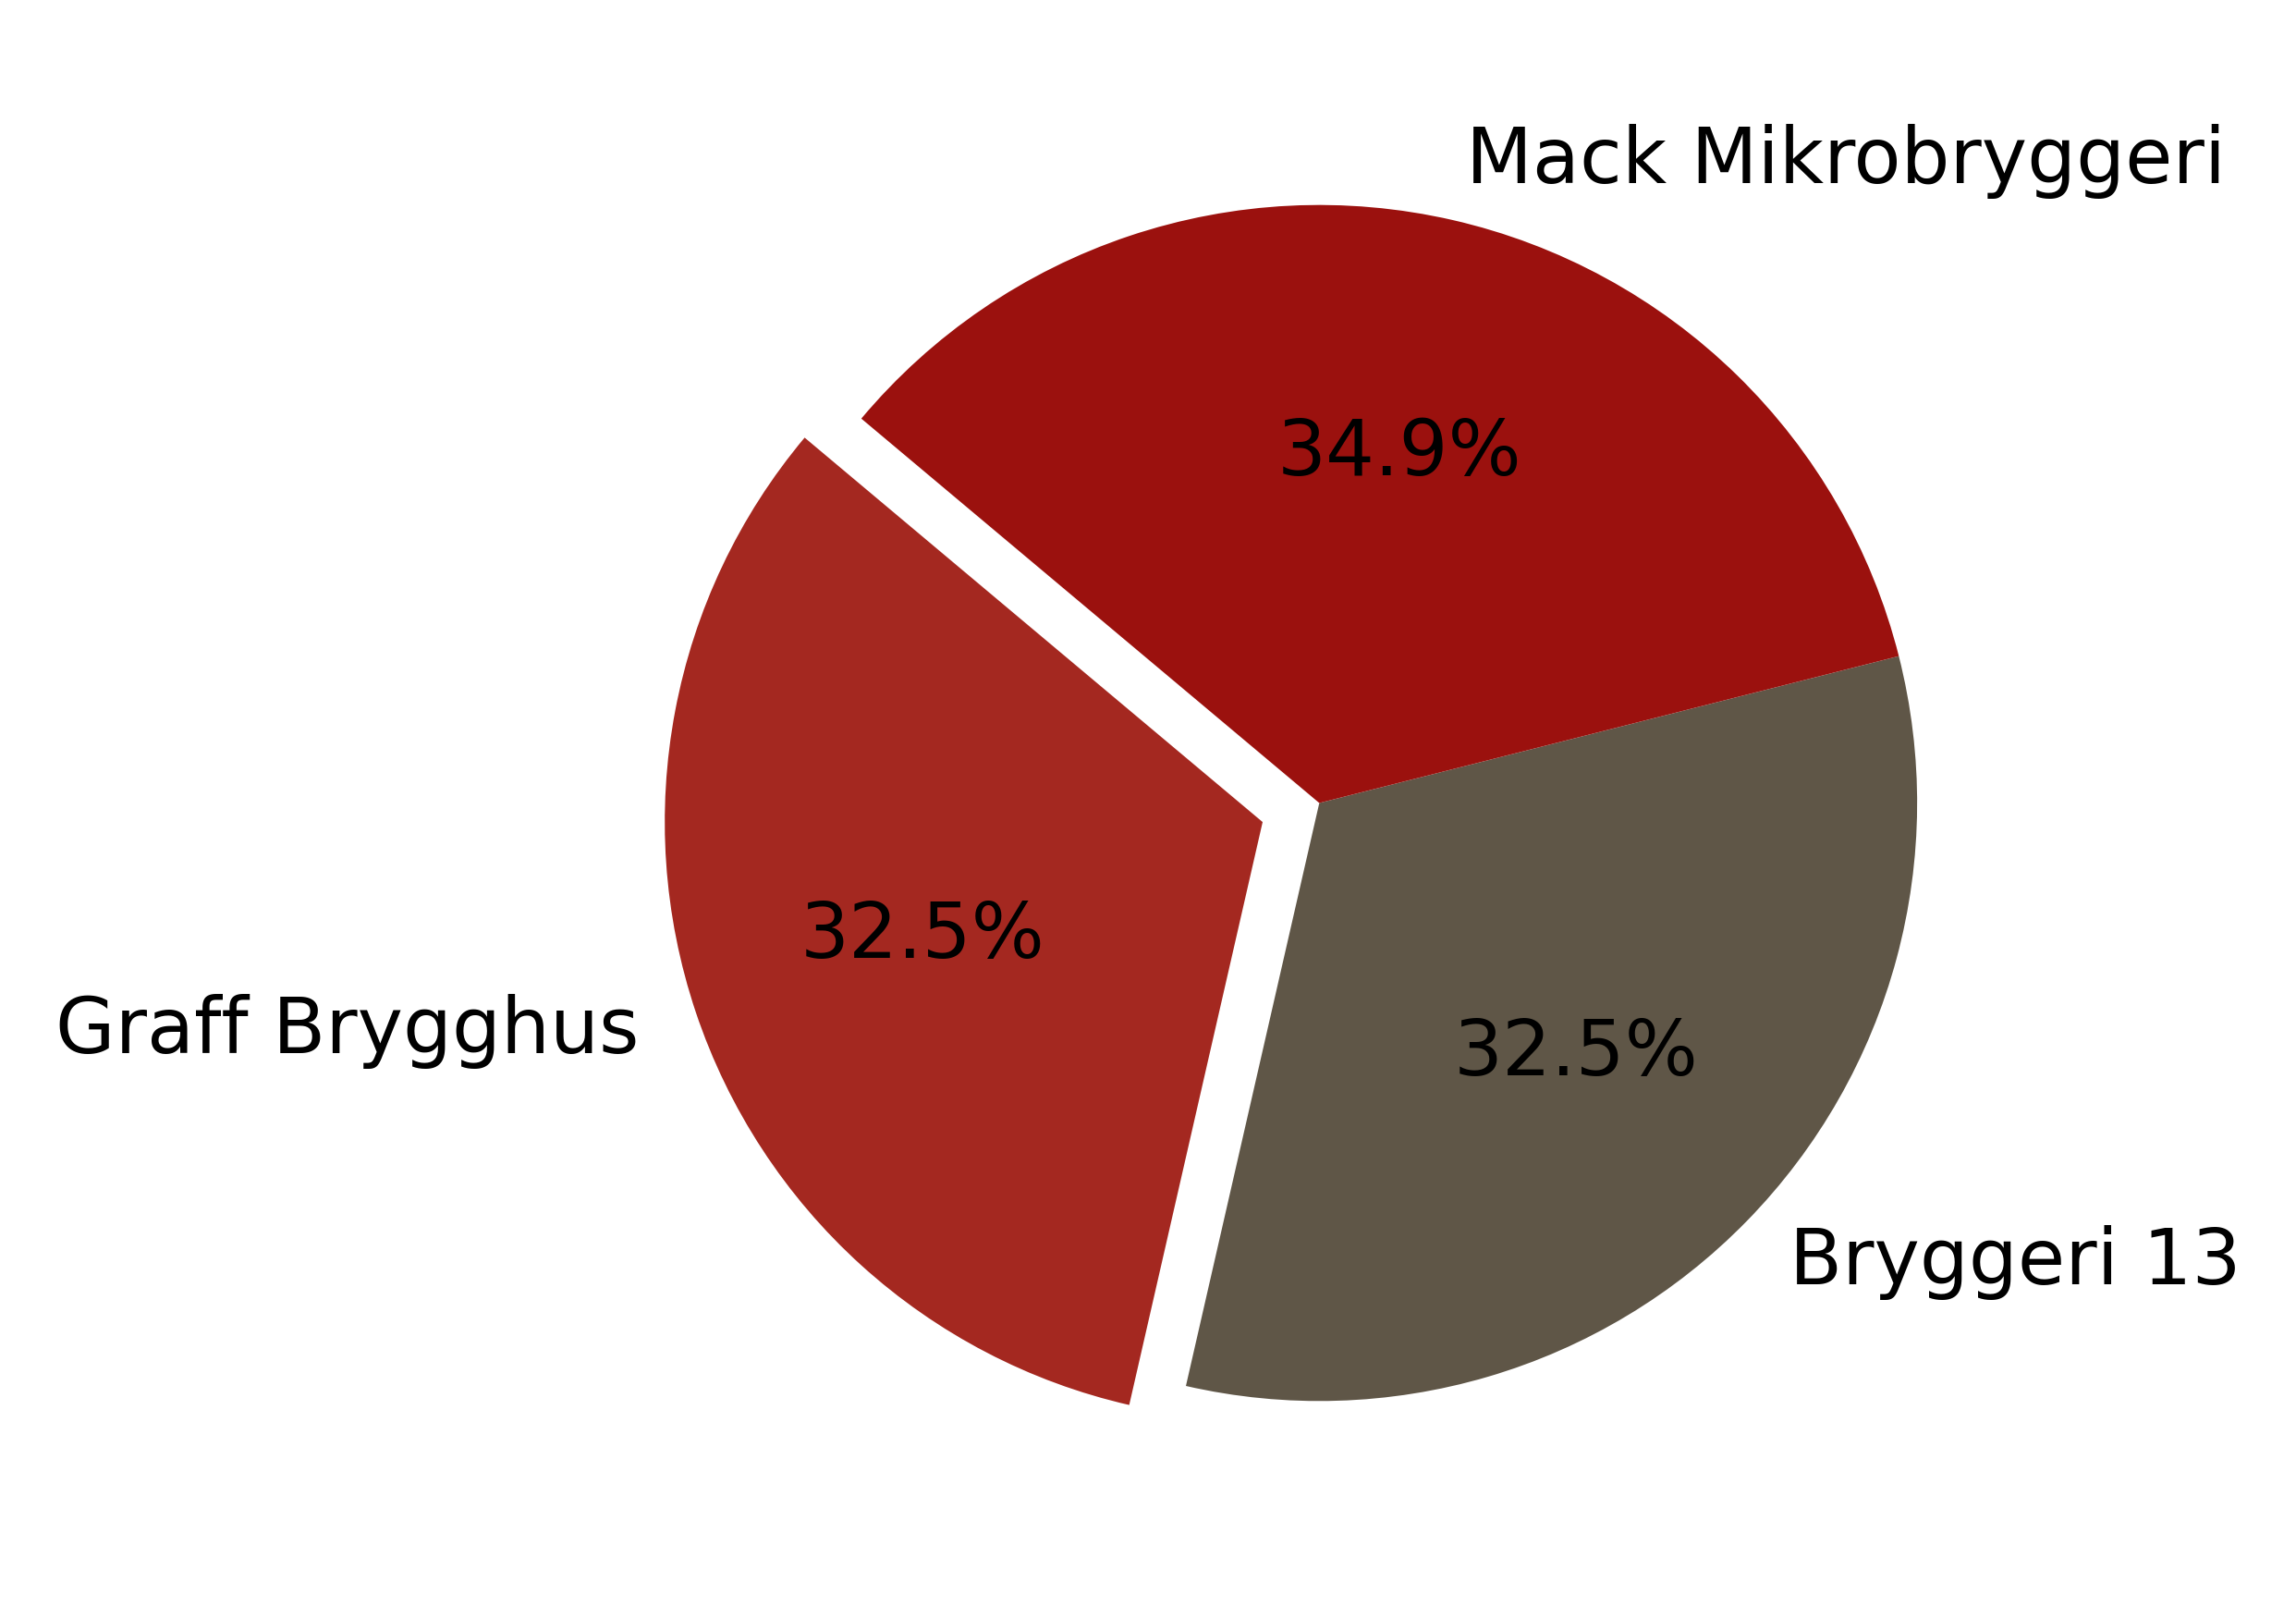
\includegraphics[width=0.5\textwidth]{dokumentobjekter/figurer/cournot_mikrobryggerier.png}
  \captionof{figure}{Cournot modell før fusjon}
  \label{fig:cournot_før_fusjon}
  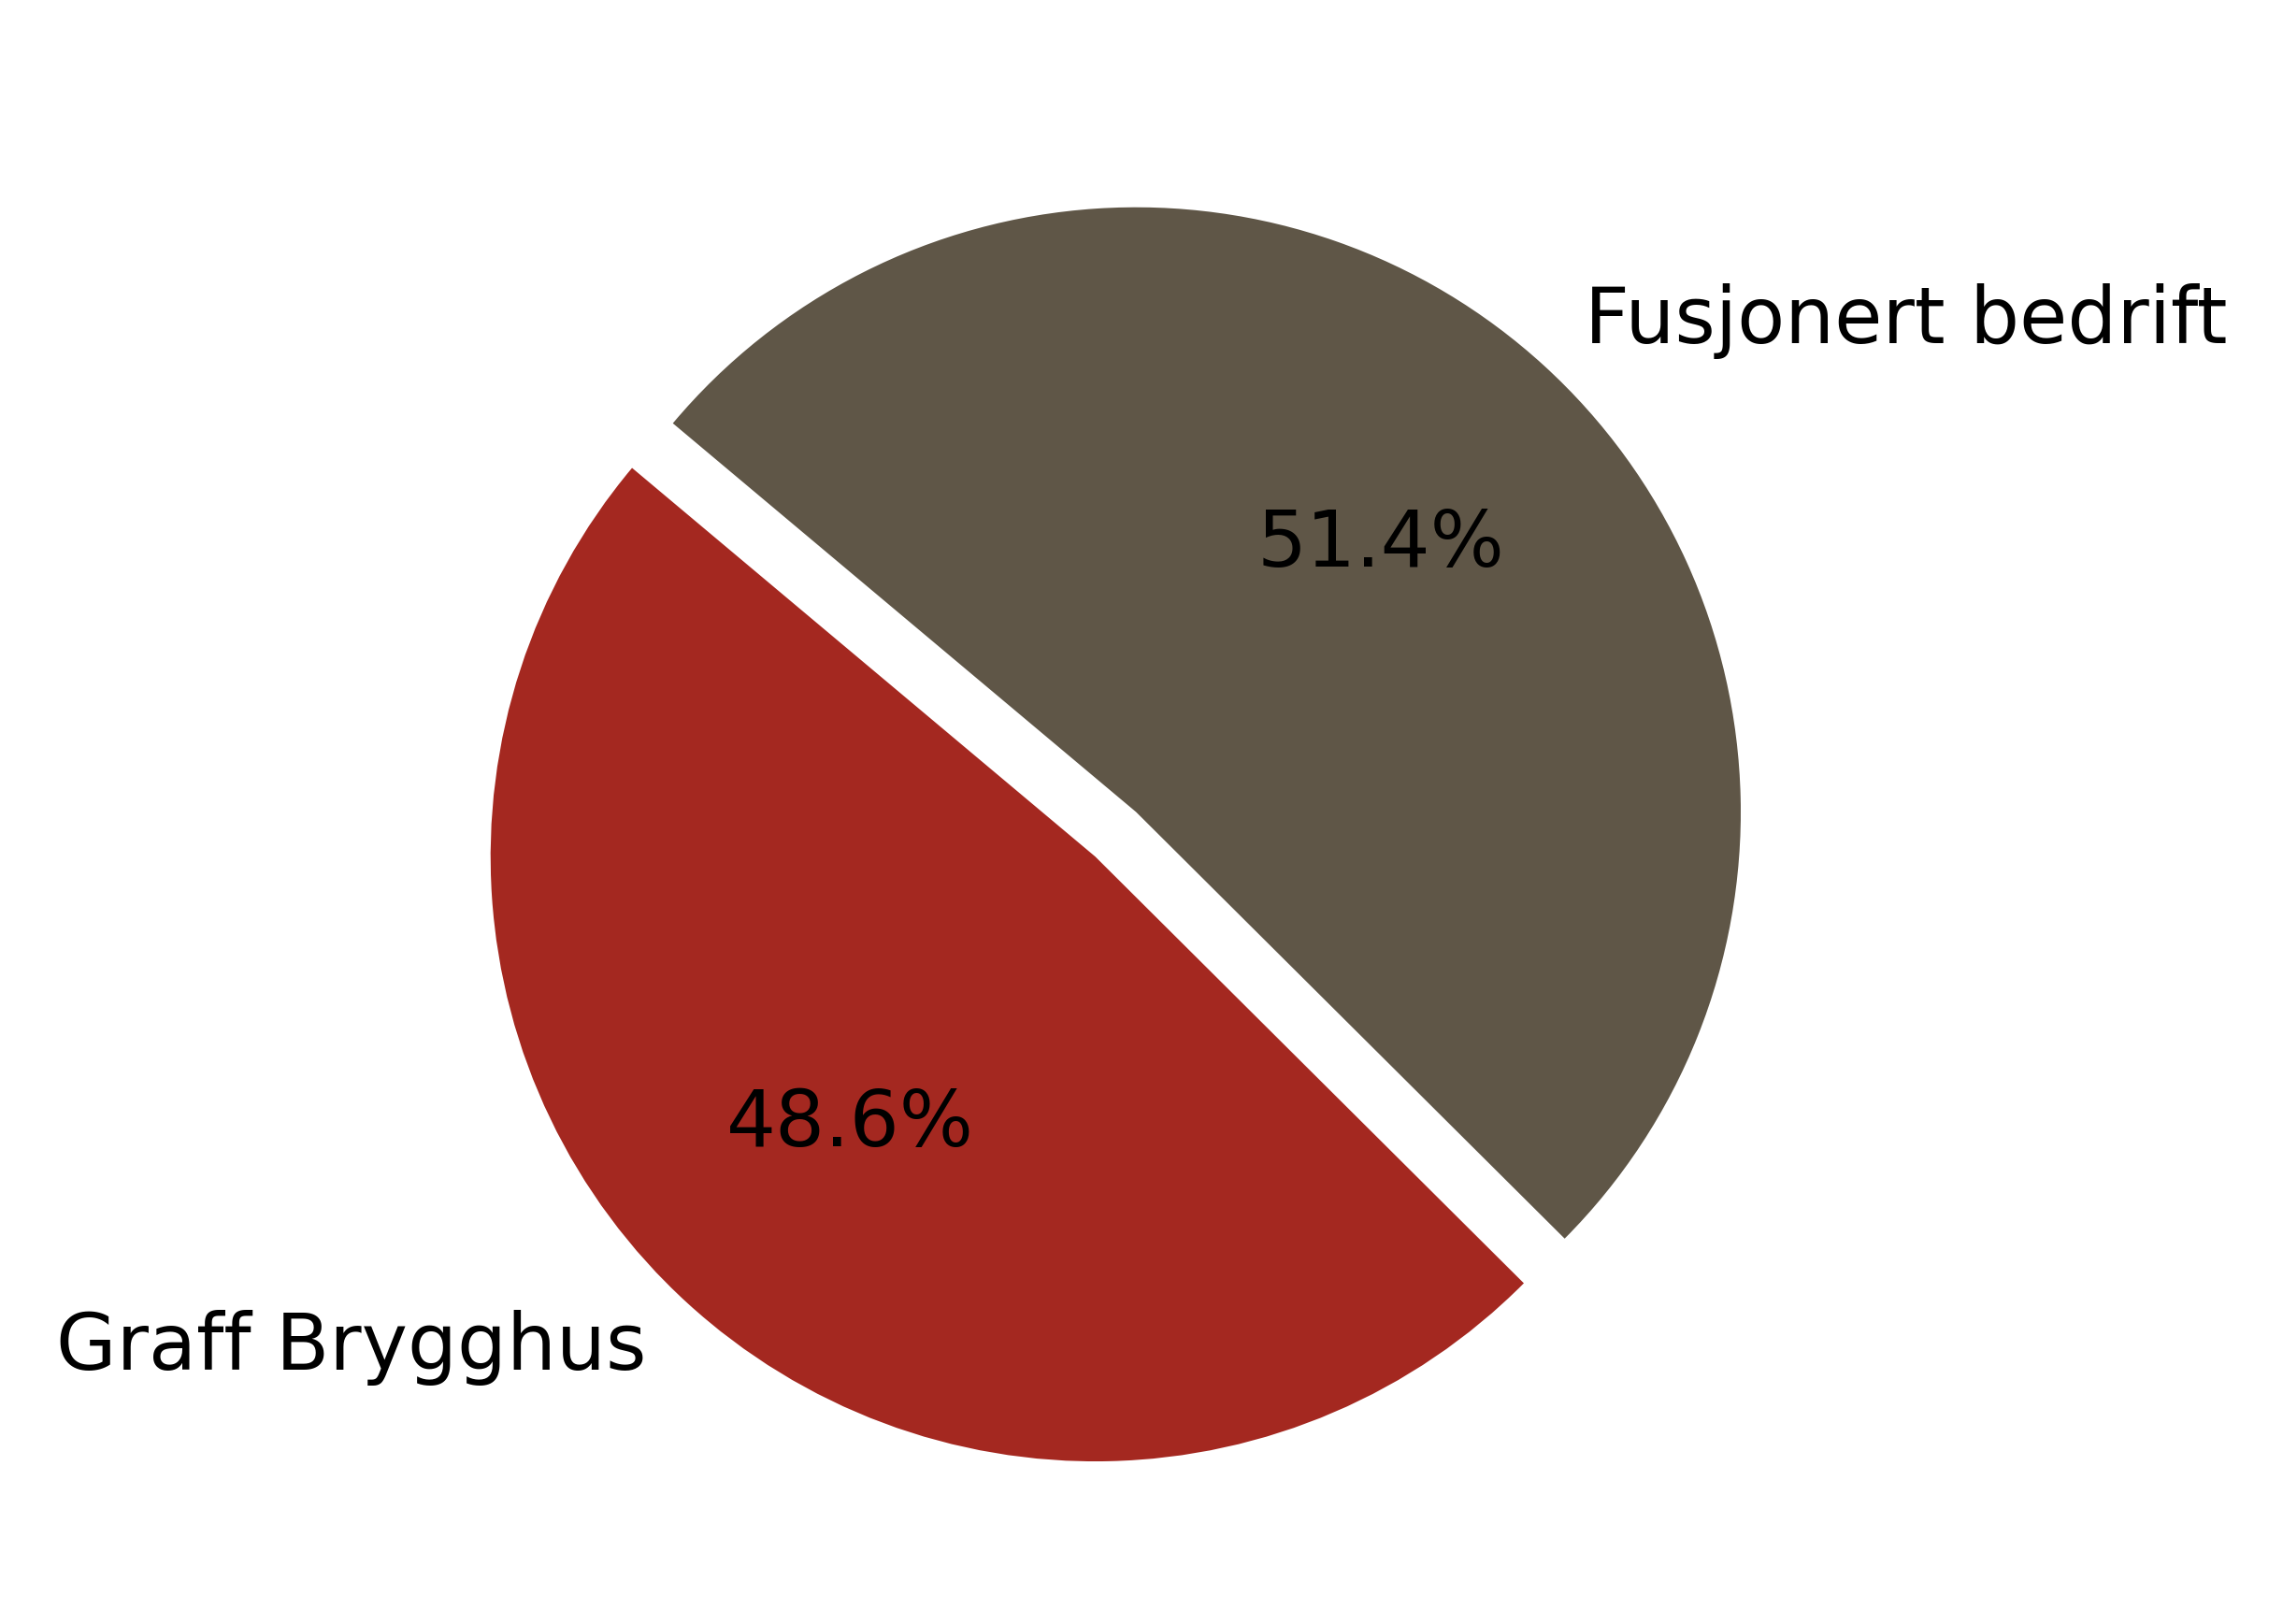
\includegraphics[width=0.5\textwidth]{dokumentobjekter/figurer/fusjonert_bedrift.png}
  \captionof{figure}{Cournot modell etter fusjon}
  \label{fig:cournot_etter_fusjon}
  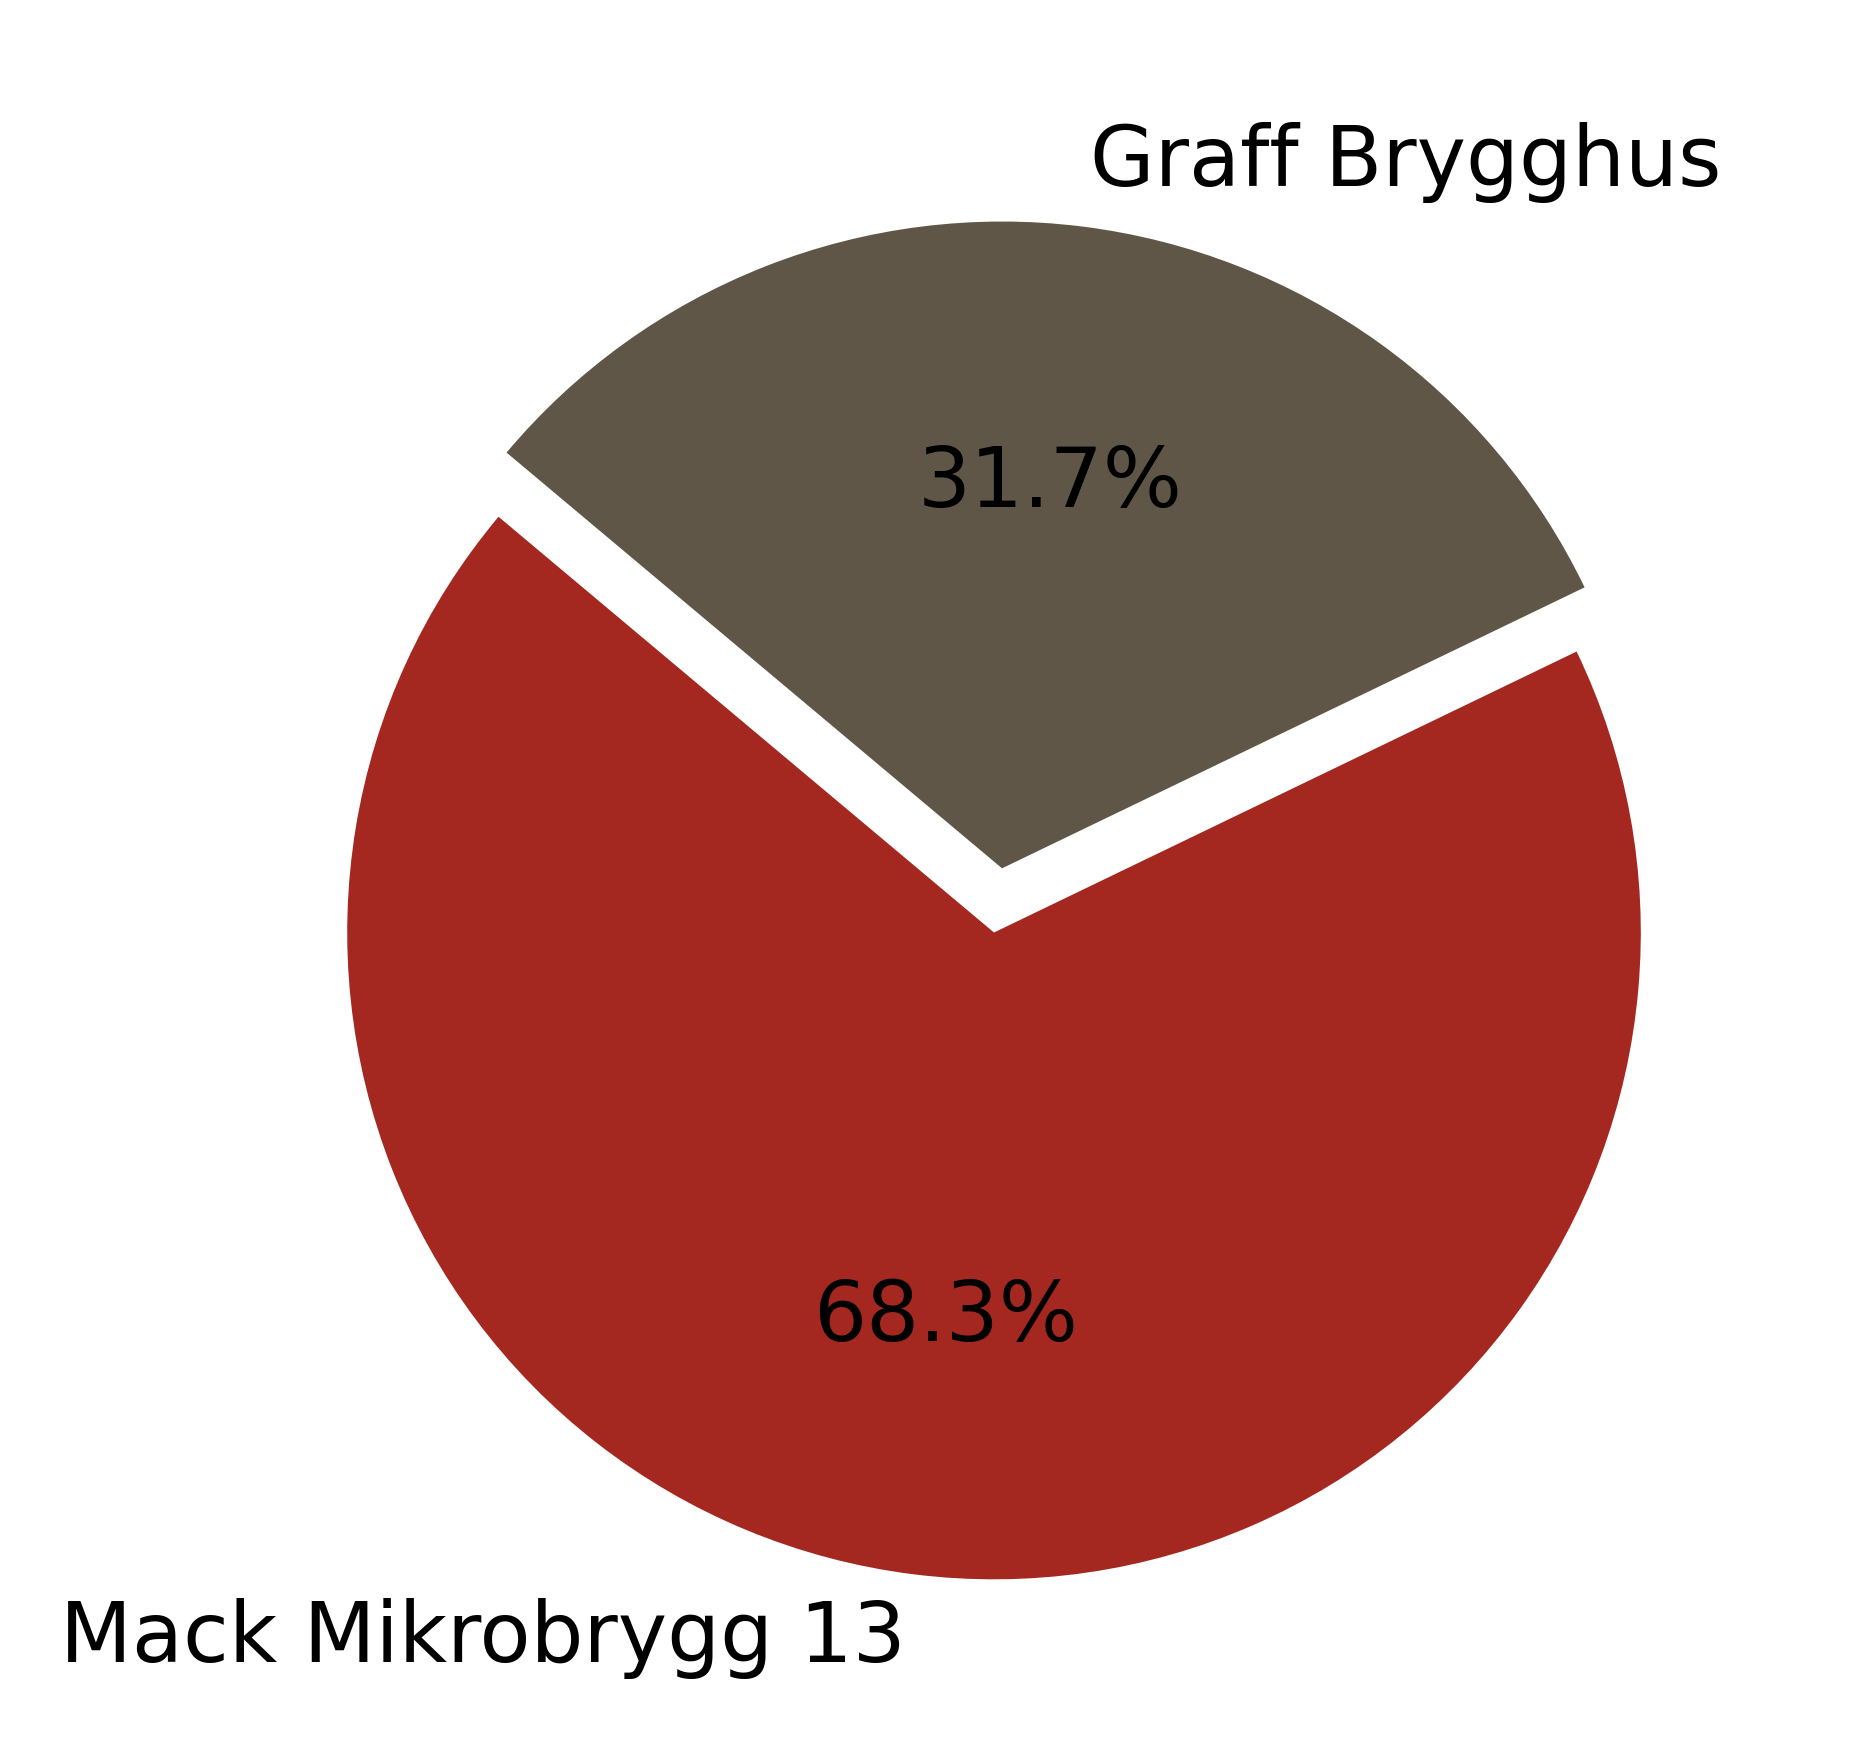
\includegraphics[width=0.5\textwidth]{dokumentobjekter/figurer/stackelberg_mack_graff.png}
  \captionof{figure}{Stackelberg modell etter fusjon}
  \label{fig:stackelberg_etter_fusjon}
  \vspace{-2.5cm}
\end{wrapfigure}

Fusjonsparadokset er enkelt forklart ved at etterspørselen etter
mikrobryggeriøl ikke endrer seg etter fusjonen og Graff som tidligere
delte markedet med to andre bryggerier, vil nå kun dele markedet med ett
bryggeri. Dette vil føre til at Graff Brygghus øker produksjonen med
\(13.15 - 10.125 =  3.025\) tusen flasker i kvantum og markedsprisen per
flaske øker fra 50.5 til 64 kr.

Fusjonsparadokset slår til her på profitten og det er Graff Brygghus som
tjener mest med en økning fra 110.062,5 kr før fusjon til 429.000 kr i
profitt. Før fusjonen hadde Bryggeri 13 og Mack Mikrobryggeri en samlet
profitt på 283.125 kr og etter fusjonen øker den til 312.250 kr opp med
29125 kr. Fusjonen vil være lønnsom for de fusjonerte partene på grunn
av at de kan flytte produksjonen til Mack hvor marginalkostnaden går
ned, dog ikke nært like mye som for Graff Brygghus.

Samfunnsøkonomisk blir kvantumet etter fusjonen ved cournot å gå ned fra
31.125 til 27.75 tusen flasker og prisen per flaske øker fra 50.5 til 64
kr. Dette vil føre til at det blir produsert mindre mikrobryggeriøl i
markedet og prisen per flaske vil øke. Og i
\autoref{fig:cournot_før_fusjon} og \autoref{fig:cournot_etter_fusjon}
kan vi se at Graff Brygghus øker sin produksjon etter fusjonen, mens
Bryggeri 13 og Mack Mikrobryggeri sin totale produksjon går ned, dog de
har større markedsandel.

\subsection{Fusjonsparadokset ved
stackelberg}\label{fusjonsparadokset-ved-stackelberg}

Siden fusjonen vil føre til at Graff Brygghus får størst profitt, så vil
det være en fordel for den nye fusjonerte bedriften å sette kvantum
først i markedet som lederbedrift ettersom de har en større
produksjonskapasitet.

Utregningen ved at Mack Mikrobryggeri og Bryggeri 13 fusjonerer og blir
en lederbedrift ligger i appendix i kode men oppsummeres i
\autoref{table:fusjon}. Og ved at Graff Brygghus er følgerbedrift så vil
profitten til Graff Brygghus gå ned til 95.015 kroner mens profitten til
den fusjonerte bedriften vil øke til 413.781 kroner, som vil gjøre det
veldig lønnsomt for de fusjonerte partene å fusjonere dersom de har
mulighet å bli lederbedrift og bestemme kvantum i markedet som vises i
\autoref{fig:stackelberg_etter_fusjon}.

\clearpage

I \autoref{table:fusjon} kan man se at det også er samfunnsøkonomisk bra
hvis Mack Mikrobryggeri og Bryggeri 13 fusjonerer og blir lederbedrift
da det vil føre til at det blir produsert mer mikrobryggeriøl i markedet
og prisen per flaske blir lavest.

\begin{table}[H]
\centering
\begin{tabular}{|c|c|c|c|}
\hline
\rowcolor{winered}
 & Cournot før fusjon & Cournot etter fusjon & Stackelberg etter fusjon \\ \hline
 \rowcolor{wesgrey}
$Q_G^*$ & 10.125 & 13.5 & 10 \\ \hline
 \rowcolor{wesgrey}
$Q_B^*$ & 10.125 & 0 & 0 \\ \hline
 \rowcolor{wesgrey}
$Q_M^*$ & 10.875 & 14.25 & 21 \\ \hline
 \rowcolor{wesgrey}
$P^*$ & 50.5 & 64 & 50 \\ \hline
 \rowcolor{wesgrey}
$\pi_G$ & 110062.5 & 429000 & 95015 \\ \hline
 \rowcolor{wesgrey}
$\pi_B$ & 110062.5 & 0 & 0 \\ \hline
 \rowcolor{wesgrey}
$\pi_M$ & 173062.5 & 312250 & 413781 \\ \hline
\end{tabular}
\caption{Optimalt kvantum, pris og profitt før og etter fusjon}
\label{table:fusjon}
\end{table}

Videre i oppgaven skal vi anta at fusjon mellom Mack Mikrobryggeri og
Bryggeri 13 blir gjennomført, og det nye selskapet vil operere under
navnet Mack Mikrobrygg 13. Markedet for produksjon av mikroøl vi da
bestå av to lokale produsenter: Mack Mikrobrygg 13 og Graff Brygghus.
For å styrke sin posisjon i markedet, investerer Graff Brygghus i nytt
og mer effektivt produksjonsutstyr, noe som reduserer deres variable
kostnader til kr 7 per flaske. Denne investeringen vil gi selskapet økte
faste kostnader på kr 200.000. Totale faste kostnader for begge
bryggeriene er da på kr 500.000 for hvert av selskapene.

I restaurantbransjen i Tromsø er Restaurant Gruppen Holdig (RGH) en
sentral aktør, som har monopol i sitt segment. RGH kjøper sitt mikroøl
fra de to lokale produsentene Mack Mikrobrygg 13 og Graff Brygghus. For
å drifte sine restauranter har RGH faste kostnader på kr 600.000.

Etterspørselen etter mikroøl i restaurantbransjen er lik:
\(P = 175 − 2Q\) hvor \(Q\) er antall solgte flasker mikroøl (antall
tusen flasker) for RGH og P er prisen for en flaske mikroøl til
sluttbruker.

For å ytterligere styrke sin posisjon i oppstrømsmarkedet, vurderer
ledelsen i Mack Mikrobrygg 13 en fusjon med konkurrenten Graff Brygghus.
Det antas at denne fusjonen ikke vil resultere i kostnadsbesparelser for
bryggeriene.

Som konsulent for styret i Mack Mikrobrygg 13, er du bedt om å analysere
markedskonsekvensene av en potensiell fusjon mellom Mack Mikrobrygg 13
og Graff Brygghus. Analysen skal omfatte en vurdering av dagens
markedstilpasning og en sammenligning med tilpasningen etter en
eventuell fusjon i oppstrømsmarkedet.

\clearpage

Basert på din analyse, vil du anbefale styret i Mack Mikrobrygg 13 å
gjennomføre fusjon med Graff Brygghus?

\subsection{Cournot modell for Graff Brygghus og Mack Mikrobrygg
13}\label{cournot-modell-for-graff-brygghus-og-mack-mikrobrygg-13}

\begin{enumerate}
\def\labelenumi{\alph{enumi})}
\setcounter{enumi}{2}
\tightlist
\item
  Hva blir de samfunnsøkonomiske konsekvensene av en fusjon mellom Mack
  Mikrobrygg 13 og Graff Brygghus.
\end{enumerate}

\clearpage

\section{Referanser}\label{referanser}

\phantomsection\label{refs}
\begin{CSLReferences}{1}{0}
\bibitem[\citeproctext]{ref-pepall_industrial_2014}
Pepall, L., Richards, D. J. \& Norman, G. (2014). \emph{Industrial
organization: Contemporary theory and empirical applications} (Fifth
edition). Wiley.

\end{CSLReferences}

\clearpage

\appendix

\section {Appendix Generell KI bruk}

I løpet av koden så kan det ses mange \# kommentarer der det er skrevet
for eks ``\#fillbetween q1 and q2''. Når jeg skriver kode i Visual
Studio Code så finnes det en plugin som heter Github Copilot. Når vi
skriver slike kommentarer så kan den foresøke å fullføre kodelinjene
mens jeg skriver de. Noen ganger klarer den det, men andre ikke. Det er
vanskelig å dokumentere hvert bruk der den er brukt siden det ``går
veldig fort'' men siden det ikke er fått på plass en slik dokumentasjon
så kan all python kode der det er brukt kommentarer antas som at det er
brukt Github Copilot. Nærmere info om dette KI verktøyet kan ses på
\url{https://github.com/features/copilot}

\clearpage

\section {Appendix Kode}

\begin{Shaded}
\begin{Highlighting}[]
\ImportTok{import}\NormalTok{ sympy }\ImportTok{as}\NormalTok{ sp}
\ImportTok{from}\NormalTok{ matplotlib }\ImportTok{import}\NormalTok{ pyplot }\ImportTok{as}\NormalTok{ plt}
\ImportTok{import}\NormalTok{ numpy }\ImportTok{as}\NormalTok{ np}

\NormalTok{q\_o, q\_c,c, a, b, pi,i, f\_k}\OperatorTok{=}\NormalTok{sp.symbols(}\StringTok{\textquotesingle{}q\_o q\_c c a b pi i f\_k\textquotesingle{}}\NormalTok{)}


\CommentTok{\# c er konstante marginalkostnader}
\CommentTok{\# a og b er parametre i etterspørselsfunksjonen som er gitt ved P = a {-} bQ}
\CommentTok{\# hvor etterspørselen er P = 990{-}1/60(Q\_o+Q\_c)}
\CommentTok{\#faste kostnader for begge bedrifter er 3 millioner}
\NormalTok{c }\OperatorTok{=} \DecValTok{50}
\NormalTok{a }\OperatorTok{=} \DecValTok{990}
\NormalTok{b }\OperatorTok{=} \DecValTok{1}\OperatorTok{/}\DecValTok{60}
\NormalTok{f\_k }\OperatorTok{=} \DecValTok{3000000}
\KeywordTok{def}\NormalTok{ P\_demand(Q,a,b):}
    \ControlFlowTok{return}\NormalTok{ a}\OperatorTok{{-}}\NormalTok{b}\OperatorTok{*}\NormalTok{Q}

\KeywordTok{def}\NormalTok{ profit(q\_o,q\_c,c,a,b):}
    \ControlFlowTok{return}\NormalTok{ (P\_demand(q\_o}\OperatorTok{+}\NormalTok{q\_c,a,b)}\OperatorTok{{-}}\NormalTok{c)}\OperatorTok{*}\NormalTok{q\_o}
\end{Highlighting}
\end{Shaded}

\begin{Shaded}
\begin{Highlighting}[]
\CommentTok{\# Deriverer profittfunksjon til Dr Choice}
\NormalTok{d\_profit2\_Q}\OperatorTok{=}\NormalTok{sp.diff(profit(q\_c,q\_o,c,a,b),q\_c)}
\NormalTok{d\_profit2\_Q}
\end{Highlighting}
\end{Shaded}

$\displaystyle - 0.0333333333333333 q_{c} - 0.0166666666666667 q_{o} + 940$

\begin{Shaded}
\begin{Highlighting}[]
\CommentTok{\# Setter den deriverte lik 0 og finner reaksjonsfunksjon til Dr choice}
\NormalTok{Q2\_sol1}\OperatorTok{=}\NormalTok{sp.solve(d\_profit2\_Q,q\_c)[}\DecValTok{0}\NormalTok{]}
\NormalTok{Q2\_sol1}
\end{Highlighting}
\end{Shaded}

$\displaystyle 28200.0 - 0.5 q_{o}$

\begin{Shaded}
\begin{Highlighting}[]
\CommentTok{\# På trinn 1 settes reaksjonsfunksjonene til Dr Choice inn i Olivita }
\CommentTok{\#sin profittfunksjon, og deriverer dette utrykket mhp q\_o}
\NormalTok{d\_profit1\_Q}\OperatorTok{=}\NormalTok{sp.diff(profit(q\_o,Q2\_sol1,c,a,b),q\_o)}
\NormalTok{d\_profit1\_Q}
\end{Highlighting}
\end{Shaded}

$\displaystyle 470.0 - 0.0166666666666667 q_{o}$

\begin{Shaded}
\begin{Highlighting}[]
\CommentTok{\# For å finne optimalt kvantum til lederbedriften (Olivita)}
\CommentTok{\#setter vi uttrykket over lik 0}
\NormalTok{Q1\_sol}\OperatorTok{=}\NormalTok{sp.solve(d\_profit1\_Q,q\_o)[}\DecValTok{0}\NormalTok{]}
\NormalTok{Q1\_sol}
\end{Highlighting}
\end{Shaded}

$\displaystyle 28200.0$

\begin{Shaded}
\begin{Highlighting}[]
\CommentTok{\# Optimalt kvantum for Dr Choice}
\NormalTok{Q2\_sol2}\OperatorTok{=}\NormalTok{Q2\_sol1.subs(\{q\_o:Q1\_sol\})}
\NormalTok{Q2\_sol2}
\end{Highlighting}
\end{Shaded}

$\displaystyle 14100.0$

\begin{Shaded}
\begin{Highlighting}[]
\KeywordTok{def}\NormalTok{ P\_demand(q1,q2):}
    \ControlFlowTok{return}\NormalTok{ a}\OperatorTok{{-}}\NormalTok{b}\OperatorTok{*}\NormalTok{(q1}\OperatorTok{+}\NormalTok{q2)}
    
\CommentTok{\# Optimal pris i sluttmarkedet:}
\NormalTok{P\_opt}\OperatorTok{=}\NormalTok{P\_demand(q\_o,q\_c).subs(\{q\_o:Q1\_sol,q\_c:Q2\_sol2\})}

\NormalTok{P\_opt}
\end{Highlighting}
\end{Shaded}

$\displaystyle 285.0$

\begin{Shaded}
\begin{Highlighting}[]
\CommentTok{\# profitt for lederbedrift (Olivita):}
\NormalTok{sp.simplify((P\_opt}\OperatorTok{{-}}\NormalTok{c)}\OperatorTok{*}\NormalTok{Q1\_sol}\OperatorTok{{-}}\NormalTok{f\_k)}
\end{Highlighting}
\end{Shaded}

$\displaystyle 3627000.0$

\begin{Shaded}
\begin{Highlighting}[]
\CommentTok{\# profitt for følgerbedrift (Dr Choice):}
\NormalTok{sp.simplify((P\_opt}\OperatorTok{{-}}\NormalTok{c)}\OperatorTok{*}\NormalTok{Q2\_sol2}\OperatorTok{{-}}\NormalTok{f\_k)}
\end{Highlighting}
\end{Shaded}

$\displaystyle 313500.0$

\begin{Shaded}
\begin{Highlighting}[]
\CommentTok{\# Lager første pai som viser hvor stort kvantum av markedet hver bedrift har ved bruk av stackelbergmodellen}
\NormalTok{labels }\OperatorTok{=} \StringTok{\textquotesingle{}Olivita\textquotesingle{}}\NormalTok{, }\StringTok{\textquotesingle{}Dr Choice\textquotesingle{}}
\NormalTok{sizes }\OperatorTok{=}\NormalTok{ [Q1\_sol,Q2\_sol2]}
\NormalTok{colors }\OperatorTok{=}\NormalTok{ [}\StringTok{\textquotesingle{}\#A42820\textquotesingle{}}\NormalTok{, }\StringTok{\textquotesingle{}\#5F5647\textquotesingle{}}\NormalTok{]}
\NormalTok{explode }\OperatorTok{=}\NormalTok{ (}\FloatTok{0.1}\NormalTok{, }\DecValTok{0}\NormalTok{)  }\CommentTok{\# explode 1st slice}
\NormalTok{plt.pie(sizes, explode}\OperatorTok{=}\NormalTok{explode, labels}\OperatorTok{=}\NormalTok{labels, colors}\OperatorTok{=}\NormalTok{colors, autopct}\OperatorTok{=}\StringTok{\textquotesingle{}}\SpecialCharTok{\%1.1f\%\%}\StringTok{\textquotesingle{}}\NormalTok{, startangle}\OperatorTok{=}\DecValTok{140}\NormalTok{)}
\NormalTok{plt.savefig(}\StringTok{\textquotesingle{}dokumentobjekter/figurer/stackelberg\_olivita\_dr\_choice.png\textquotesingle{}}\NormalTok{, bbox\_inches}\OperatorTok{=}\StringTok{\textquotesingle{}tight\textquotesingle{}}\NormalTok{, dpi}\OperatorTok{=}\DecValTok{600}\NormalTok{)}
\end{Highlighting}
\end{Shaded}

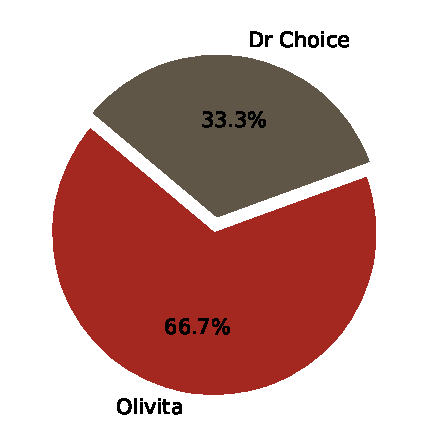
\includegraphics{Kandidatnummer_30_mappeoppgave_2_SOK_2030_files/figure-pdf/cell-11-output-1.pdf}

\begin{Shaded}
\begin{Highlighting}[]
\CommentTok{\# regner cournot likevekt}
\NormalTok{q1, q2,c1,c2, a, b}\OperatorTok{=}\NormalTok{sp.symbols(}\StringTok{\textquotesingle{}q1 q2 c1 c2 a b\textquotesingle{}}\NormalTok{)}

\NormalTok{a }\OperatorTok{=} \DecValTok{990}
\NormalTok{b }\OperatorTok{=} \DecValTok{1}\OperatorTok{/}\DecValTok{60}
\NormalTok{c }\OperatorTok{=} \DecValTok{50}
\KeywordTok{def}\NormalTok{ P\_demand(Q,a,b):}
    \ControlFlowTok{return}\NormalTok{ a}\OperatorTok{{-}}\NormalTok{b}\OperatorTok{*}\NormalTok{Q}

\KeywordTok{def}\NormalTok{ profit(q1,q2,c,a,b):}
    \ControlFlowTok{return}\NormalTok{ (P\_demand(q1}\OperatorTok{+}\NormalTok{q2,a,b)}\OperatorTok{{-}}\NormalTok{c)}\OperatorTok{*}\NormalTok{q1}
\end{Highlighting}
\end{Shaded}

\begin{Shaded}
\begin{Highlighting}[]
\NormalTok{d\_profit1\_Q}\OperatorTok{=}\NormalTok{sp.diff(profit(q1,q2,c,a,b),q1)}
\NormalTok{d\_profit2\_Q}\OperatorTok{=}\NormalTok{sp.diff(profit(q2,q1,c,a,b),q2)}

\NormalTok{display(d\_profit1\_Q)}
\NormalTok{display(d\_profit2\_Q)}
\end{Highlighting}
\end{Shaded}

$\displaystyle - 0.0333333333333333 q_{1} - 0.0166666666666667 q_{2} + 940$

$\displaystyle - 0.0166666666666667 q_{1} - 0.0333333333333333 q_{2} + 940$

\begin{Shaded}
\begin{Highlighting}[]
\NormalTok{sol}\OperatorTok{=}\NormalTok{sp.solve([d\_profit1\_Q,d\_profit2\_Q],[q1,q2])}

\NormalTok{display((sol[q1]))}
\NormalTok{display((sol[q2]))}
\end{Highlighting}
\end{Shaded}

$\displaystyle 18800.0$

$\displaystyle 18800.0$

\begin{Shaded}
\begin{Highlighting}[]
\NormalTok{sol}\OperatorTok{=}\NormalTok{sp.solve([d\_profit1\_Q,d\_profit2\_Q],[q1,q2])}

\NormalTok{Q1\_sol }\OperatorTok{=}\NormalTok{sp.simplify((sol[q1]))}
\NormalTok{Q1\_sol}
\end{Highlighting}
\end{Shaded}

$\displaystyle 18800.0$

\begin{Shaded}
\begin{Highlighting}[]
\NormalTok{Q2\_sol }\OperatorTok{=}\NormalTok{sp.simplify((sol[q1]))}
\NormalTok{Q2\_sol}
\end{Highlighting}
\end{Shaded}

$\displaystyle 18800.0$

\begin{Shaded}
\begin{Highlighting}[]
\KeywordTok{def}\NormalTok{ P\_demand(q1,q2):}
    \ControlFlowTok{return}\NormalTok{ a}\OperatorTok{{-}}\NormalTok{b}\OperatorTok{*}\NormalTok{(q1}\OperatorTok{+}\NormalTok{q2)}
\CommentTok{\# Optimal pris i sluttmarkedet:}
\NormalTok{P\_opt}\OperatorTok{=}\NormalTok{P\_demand(q1,q2).subs(\{q1:sol[q1],q2:sol[q2]\})}
\NormalTok{P\_opt}
\end{Highlighting}
\end{Shaded}

$\displaystyle 363.333333333333$

\begin{Shaded}
\begin{Highlighting}[]
\CommentTok{\# profitt for lederbedrift (Olivita):}
\NormalTok{sp.simplify((P\_opt}\OperatorTok{{-}}\NormalTok{c)}\OperatorTok{*}\NormalTok{sol[q1]}\OperatorTok{{-}}\NormalTok{f\_k)}
\end{Highlighting}
\end{Shaded}

$\displaystyle 2890666.66666667$

\begin{Shaded}
\begin{Highlighting}[]
\CommentTok{\# Lager andre pai som viser hvor stor andel av markedet hver bedrift har ved bruk av cournot modellen}
\NormalTok{sizes }\OperatorTok{=}\NormalTok{ [Q1\_sol,Q2\_sol]}
\NormalTok{plt.pie(sizes, explode }\OperatorTok{=}\NormalTok{ explode,labels}\OperatorTok{=}\NormalTok{labels, colors}\OperatorTok{=}\NormalTok{colors, autopct}\OperatorTok{=}\StringTok{\textquotesingle{}}\SpecialCharTok{\%1.1f\%\%}\StringTok{\textquotesingle{}}\NormalTok{, startangle}\OperatorTok{=}\DecValTok{140}\NormalTok{)}
\NormalTok{plt.savefig(}\StringTok{\textquotesingle{}dokumentobjekter/figurer/cournot\_olivita\_dr\_choice.png\textquotesingle{}}\NormalTok{, bbox\_inches}\OperatorTok{=}\StringTok{\textquotesingle{}tight\textquotesingle{}}\NormalTok{, dpi}\OperatorTok{=}\DecValTok{600}\NormalTok{)}
\end{Highlighting}
\end{Shaded}

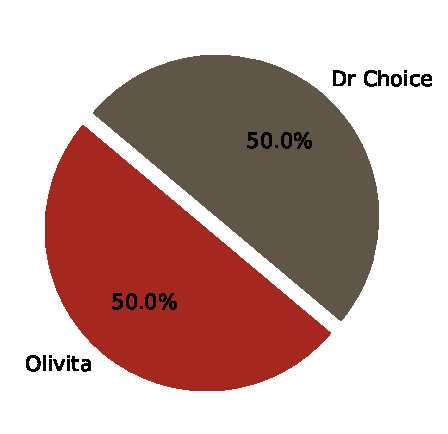
\includegraphics{Kandidatnummer_30_mappeoppgave_2_SOK_2030_files/figure-pdf/cell-19-output-1.pdf}

\begin{Shaded}
\begin{Highlighting}[]
\CommentTok{\# Starter på oppgave 2, regner på nytt cournot for mikroøl}
\CommentTok{\# q\_g er graffi, q\_b er bryggeri 13 og q\_m er mack mikrobryggeri}

\CommentTok{\# regner cournot likevekt}
\NormalTok{q\_g, q\_b, q\_m,c\_g,c\_b,c\_m, a, b, f\_k,c}\OperatorTok{=}\NormalTok{sp.symbols(}\StringTok{\textquotesingle{}q\_g q\_b q\_m c\_g c\_b c\_m a b f\_k c\textquotesingle{}}\NormalTok{)}

\NormalTok{a }\OperatorTok{=} \DecValTok{175}
\NormalTok{b }\OperatorTok{=} \DecValTok{4}
\NormalTok{c\_g }\OperatorTok{=} \DecValTok{10}
\NormalTok{c\_b }\OperatorTok{=} \DecValTok{10}
\NormalTok{c\_m }\OperatorTok{=} \DecValTok{7}
\NormalTok{f\_k }\OperatorTok{=} \DecValTok{300000}
\KeywordTok{def}\NormalTok{ P\_demand(Q,a,b):}
    \ControlFlowTok{return}\NormalTok{ a}\OperatorTok{{-}}\NormalTok{b}\OperatorTok{*}\NormalTok{Q}

\KeywordTok{def}\NormalTok{ profit(q\_g,q\_b,q\_m,c,a,b):}
    \ControlFlowTok{return}\NormalTok{ (P\_demand(q\_g}\OperatorTok{+}\NormalTok{q\_b}\OperatorTok{+}\NormalTok{q\_m,a,b)}\OperatorTok{{-}}\NormalTok{c)}\OperatorTok{*}\NormalTok{q\_g}
\end{Highlighting}
\end{Shaded}

\begin{Shaded}
\begin{Highlighting}[]
\NormalTok{d\_profit1\_Q}\OperatorTok{=}\NormalTok{sp.diff(profit(q\_g,q\_b,q\_m,c\_g,a,b),q\_g)}
\NormalTok{d\_profit2\_Q}\OperatorTok{=}\NormalTok{sp.diff(profit(q\_b,q\_g, q\_m,c\_b,a,b),q\_b)}
\NormalTok{d\_profit3\_Q}\OperatorTok{=}\NormalTok{sp.diff(profit(q\_m,q\_g,q\_b,c\_m,a,b),q\_m)}


\NormalTok{display(d\_profit1\_Q)}
\NormalTok{display(d\_profit2\_Q)}
\NormalTok{display(d\_profit3\_Q)}
\end{Highlighting}
\end{Shaded}

$\displaystyle - 4 q_{b} - 8 q_{g} - 4 q_{m} + 165$

$\displaystyle - 8 q_{b} - 4 q_{g} - 4 q_{m} + 165$

$\displaystyle - 4 q_{b} - 4 q_{g} - 8 q_{m} + 168$

\begin{Shaded}
\begin{Highlighting}[]
\CommentTok{\# Tallene blir i tusener}

\NormalTok{sol}\OperatorTok{=}\NormalTok{sp.solve([d\_profit1\_Q,d\_profit2\_Q,d\_profit3\_Q],[q\_g,q\_b,q\_m])}

\CommentTok{\# Kvantum til Graff brygghus}
\NormalTok{display((sol[q\_g]))}
\CommentTok{\# Kvantum til Bryggeri 13}
\NormalTok{display((sol[q\_b]))}
\CommentTok{\# Kvantum til Mack mikrobryggeri}
\NormalTok{display((sol[q\_m]))}
\end{Highlighting}
\end{Shaded}

$\displaystyle \frac{81}{8}$

$\displaystyle \frac{81}{8}$

$\displaystyle \frac{87}{8}$

\begin{Shaded}
\begin{Highlighting}[]
\KeywordTok{def}\NormalTok{ P\_demand(q\_g,q\_b,q\_m):}
    \ControlFlowTok{return}\NormalTok{ a}\OperatorTok{{-}}\NormalTok{b}\OperatorTok{*}\NormalTok{(q\_g}\OperatorTok{+}\NormalTok{q\_b}\OperatorTok{+}\NormalTok{q\_m)}

\CommentTok{\# Optimal pris i sluttmarkedet:}
\NormalTok{P\_opt}\OperatorTok{=}\NormalTok{P\_demand(q\_g,q\_b,q\_m).subs(\{q\_g:sol[q\_g],q\_b:sol[q\_b],q\_m:sol[q\_m]\})}

\NormalTok{P\_opt}
\end{Highlighting}
\end{Shaded}

$\displaystyle \frac{101}{2}$

\begin{Shaded}
\begin{Highlighting}[]
\CommentTok{\# Husk å gange med 1000 for å finne profitt siden tall er oppgitt i tusen}

\CommentTok{\# profitt for (Graff brygghus):}
\NormalTok{Graff}\OperatorTok{=}\NormalTok{ sp.simplify((P\_opt}\OperatorTok{{-}}\NormalTok{c\_g)}\OperatorTok{*}\NormalTok{(sol[q\_g]}\OperatorTok{*}\DecValTok{1000}\NormalTok{)}\OperatorTok{{-}}\NormalTok{f\_k)}
\NormalTok{display(Graff)}
\CommentTok{\# profitt for Bryggeri 13:}
\NormalTok{Bryggeri\_13}\OperatorTok{=}\NormalTok{ sp.simplify((P\_opt}\OperatorTok{{-}}\NormalTok{c\_b)}\OperatorTok{*}\NormalTok{(sol[q\_b]}\OperatorTok{*}\DecValTok{1000}\NormalTok{)}\OperatorTok{{-}}\NormalTok{f\_k)}

\CommentTok{\# profitt for Mack mikrobryggeri:}
\NormalTok{Mack }\OperatorTok{=}\NormalTok{ sp.simplify((P\_opt}\OperatorTok{{-}}\NormalTok{c\_m)}\OperatorTok{*}\NormalTok{(sol[q\_m]}\OperatorTok{*}\DecValTok{1000}\NormalTok{)}\OperatorTok{{-}}\NormalTok{f\_k)}

\NormalTok{display(Bryggeri\_13)}
\NormalTok{display(Mack)}

\CommentTok{\#Profitt for bryggeri 13 og mack før fusjon}
\NormalTok{Mack}\OperatorTok{+}\NormalTok{Bryggeri\_13}
\end{Highlighting}
\end{Shaded}

$\displaystyle \frac{220125}{2}$

$\displaystyle \frac{220125}{2}$

$\displaystyle \frac{346125}{2}$

$\displaystyle 283125$

\begin{Shaded}
\begin{Highlighting}[]
\CommentTok{\# Oppgave 2 figur for mikrobryggeriene}
\NormalTok{labels }\OperatorTok{=} \StringTok{\textquotesingle{}Graff Brygghus\textquotesingle{}}\NormalTok{, }\StringTok{\textquotesingle{}Bryggeri 13\textquotesingle{}}\NormalTok{, }\StringTok{\textquotesingle{}Mack Mikrobryggeri\textquotesingle{}}
\NormalTok{sizes }\OperatorTok{=}\NormalTok{ [sol[q\_g],sol[q\_b],sol[q\_m]]}
\NormalTok{colors }\OperatorTok{=}\NormalTok{ [}\StringTok{\textquotesingle{}\#A42820\textquotesingle{}}\NormalTok{, }\StringTok{\textquotesingle{}\#5F5647\textquotesingle{}}\NormalTok{, }\StringTok{\textquotesingle{}\#9B110E\textquotesingle{}}\NormalTok{]}
\NormalTok{explode }\OperatorTok{=}\NormalTok{ (}\FloatTok{0.1}\NormalTok{, }\DecValTok{0}\NormalTok{, }\DecValTok{0}\NormalTok{)  }\CommentTok{\# explode 1st slice}
\NormalTok{plt.pie(sizes, explode}\OperatorTok{=}\NormalTok{explode, labels}\OperatorTok{=}\NormalTok{labels, colors}\OperatorTok{=}\NormalTok{colors, autopct}\OperatorTok{=}\StringTok{\textquotesingle{}}\SpecialCharTok{\%1.1f\%\%}\StringTok{\textquotesingle{}}\NormalTok{, startangle}\OperatorTok{=}\DecValTok{140}\NormalTok{)}
\NormalTok{plt.savefig(}\StringTok{\textquotesingle{}dokumentobjekter/figurer/cournot\_mikrobryggerier.png\textquotesingle{}}\NormalTok{, bbox\_inches}\OperatorTok{=}\StringTok{\textquotesingle{}tight\textquotesingle{}}\NormalTok{, dpi}\OperatorTok{=}\DecValTok{600}\NormalTok{)}
\end{Highlighting}
\end{Shaded}

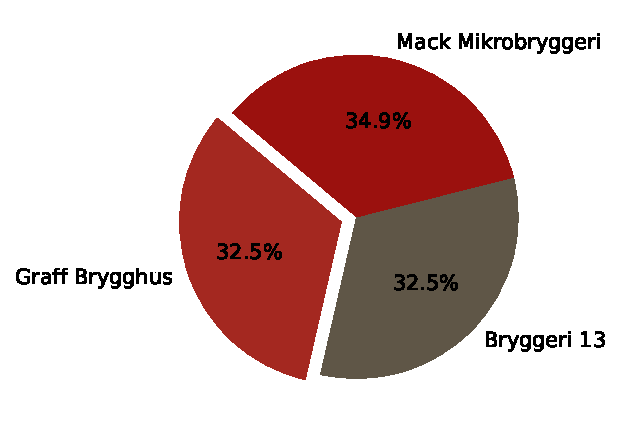
\includegraphics{Kandidatnummer_30_mappeoppgave_2_SOK_2030_files/figure-pdf/cell-25-output-1.pdf}

\begin{Shaded}
\begin{Highlighting}[]
\CommentTok{\# Fusjonerer to asymmetriske cournot bedrifter Mack mikrobryggeri og Bryggeri 13}

\CommentTok{\# Oppgave 2a}
\CommentTok{\# q\_g er kvantum til Graff brygghus}
\CommentTok{\# q\_bm blir kvantum til den fusjonerte bedriften}
\CommentTok{\# ny fk for den fusjonerte bedriften blir 500 000}

\CommentTok{\# regner cournot likevekt}
\NormalTok{q\_g, q\_bm,c\_g,c\_bm, a, b, f\_k,c, f\_k\_bm}\OperatorTok{=}\NormalTok{sp.symbols(}\StringTok{\textquotesingle{}q\_g q\_bm c\_g c\_bm a b f\_k c f\_k\_bm\textquotesingle{}}\NormalTok{)}

\NormalTok{a }\OperatorTok{=} \DecValTok{175}
\NormalTok{b }\OperatorTok{=} \DecValTok{4}
\NormalTok{c\_g }\OperatorTok{=} \DecValTok{10}
\NormalTok{c\_bm }\OperatorTok{=} \DecValTok{7}
\NormalTok{f\_k }\OperatorTok{=} \DecValTok{300000}
\NormalTok{f\_k\_bm }\OperatorTok{=} \DecValTok{500000}
\KeywordTok{def}\NormalTok{ P\_demand(Q,a,b):}
    \ControlFlowTok{return}\NormalTok{ a}\OperatorTok{{-}}\NormalTok{b}\OperatorTok{*}\NormalTok{Q}

\KeywordTok{def}\NormalTok{ profit(q\_g,q\_bm,c,a,b):}
    \ControlFlowTok{return}\NormalTok{ (P\_demand(q\_g}\OperatorTok{+}\NormalTok{q\_bm,a,b)}\OperatorTok{{-}}\NormalTok{c)}\OperatorTok{*}\NormalTok{q\_g}
\end{Highlighting}
\end{Shaded}

\begin{Shaded}
\begin{Highlighting}[]
\NormalTok{d\_profit1\_Q}\OperatorTok{=}\NormalTok{sp.diff(profit(q\_g,q\_bm,c\_g,a,b),q\_g)}
\NormalTok{d\_profit2\_Q}\OperatorTok{=}\NormalTok{sp.diff(profit(q\_bm,q\_g,c\_bm,a,b),q\_bm)}


\NormalTok{display(d\_profit1\_Q)}
\NormalTok{display(d\_profit2\_Q)}
\end{Highlighting}
\end{Shaded}

$\displaystyle - 4 q_{bm} - 8 q_{g} + 165$

$\displaystyle - 8 q_{bm} - 4 q_{g} + 168$

\begin{Shaded}
\begin{Highlighting}[]
\CommentTok{\# Kvantum er i tusener}

\NormalTok{sol}\OperatorTok{=}\NormalTok{sp.solve([d\_profit1\_Q,d\_profit2\_Q],[q\_g,q\_bm])}

\CommentTok{\# Kvantum til Graff brygghus}
\NormalTok{display(}\BuiltInTok{float}\NormalTok{(sol[q\_g]))}
\CommentTok{\# Kvantum til fusjonert bedrift}
\NormalTok{display(}\BuiltInTok{float}\NormalTok{(sol[q\_bm]))}
\end{Highlighting}
\end{Shaded}

\begin{verbatim}
13.5
\end{verbatim}

\begin{verbatim}
14.25
\end{verbatim}

\begin{Shaded}
\begin{Highlighting}[]
\KeywordTok{def}\NormalTok{ P\_demand(q\_g,q\_bm):}
    \ControlFlowTok{return}\NormalTok{ a}\OperatorTok{{-}}\NormalTok{b}\OperatorTok{*}\NormalTok{(q\_g}\OperatorTok{+}\NormalTok{q\_bm)}

\CommentTok{\# Optimal pris i sluttmarkedet:}
\NormalTok{P\_opt}\OperatorTok{=}\NormalTok{P\_demand(q\_g,q\_bm).subs(\{q\_g:sol[q\_g],q\_bm:sol[q\_bm]\})}

\CommentTok{\# Optimal sluttpris }
\NormalTok{P\_opt}
\end{Highlighting}
\end{Shaded}

$\displaystyle 64$

\begin{Shaded}
\begin{Highlighting}[]
\CommentTok{\# profitt for (Graff brygghus):}
\NormalTok{display(sp.simplify((P\_opt}\OperatorTok{{-}}\NormalTok{c\_g)}\OperatorTok{*}\NormalTok{(sol[q\_g]}\OperatorTok{*}\DecValTok{1000}\NormalTok{)}\OperatorTok{{-}}\NormalTok{f\_k))}

\CommentTok{\# profitt for fusjonert bedrift}
\NormalTok{display(sp.simplify((P\_opt}\OperatorTok{{-}}\NormalTok{c\_bm)}\OperatorTok{*}\NormalTok{(sol[q\_bm]}\OperatorTok{*}\DecValTok{1000}\NormalTok{)}\OperatorTok{{-}}\NormalTok{f\_k\_bm))}
\end{Highlighting}
\end{Shaded}

$\displaystyle 429000$

$\displaystyle 312250$

\begin{Shaded}
\begin{Highlighting}[]
\CommentTok{\# Figur for markedet etter fusjon}

\NormalTok{labels }\OperatorTok{=} \StringTok{\textquotesingle{}Graff Brygghus\textquotesingle{}}\NormalTok{, }\StringTok{\textquotesingle{}Fusjonert bedrift\textquotesingle{}}
\NormalTok{sizes }\OperatorTok{=}\NormalTok{ [sol[q\_g],sol[q\_bm]]}
\NormalTok{colors }\OperatorTok{=}\NormalTok{ [}\StringTok{\textquotesingle{}\#A42820\textquotesingle{}}\NormalTok{, }\StringTok{\textquotesingle{}\#5F5647\textquotesingle{}}\NormalTok{]}
\NormalTok{explode }\OperatorTok{=}\NormalTok{ (}\FloatTok{0.1}\NormalTok{, }\DecValTok{0}\NormalTok{)  }\CommentTok{\# explode 1st slice}
\NormalTok{plt.pie(sizes, explode}\OperatorTok{=}\NormalTok{explode, labels}\OperatorTok{=}\NormalTok{labels, colors}\OperatorTok{=}\NormalTok{colors, autopct}\OperatorTok{=}\StringTok{\textquotesingle{}}\SpecialCharTok{\%1.1f\%\%}\StringTok{\textquotesingle{}}\NormalTok{, startangle}\OperatorTok{=}\DecValTok{140}\NormalTok{)}
\NormalTok{plt.savefig(}\StringTok{\textquotesingle{}dokumentobjekter/figurer/fusjonert\_bedrift.png\textquotesingle{}}\NormalTok{,bbox\_inches}\OperatorTok{=}\StringTok{\textquotesingle{}tight\textquotesingle{}}\NormalTok{, dpi}\OperatorTok{=}\DecValTok{600}\NormalTok{)}
\end{Highlighting}
\end{Shaded}

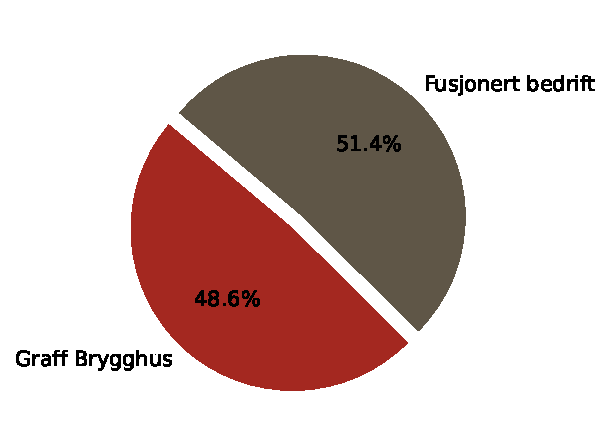
\includegraphics{Kandidatnummer_30_mappeoppgave_2_SOK_2030_files/figure-pdf/cell-31-output-1.pdf}

\begin{Shaded}
\begin{Highlighting}[]
\NormalTok{q1, q2,c, a, b, pi,i}\OperatorTok{=}\NormalTok{sp.symbols(}\StringTok{\textquotesingle{}q1 q2 c a b pi i\textquotesingle{}}\NormalTok{)}

\NormalTok{a }\OperatorTok{=} \DecValTok{175}
\NormalTok{b }\OperatorTok{=} \DecValTok{4}
\NormalTok{c }\OperatorTok{=} \DecValTok{10}


\KeywordTok{def}\NormalTok{ P\_demand(Q,a,b):}
    \ControlFlowTok{return}\NormalTok{ a}\OperatorTok{{-}}\NormalTok{b}\OperatorTok{*}\NormalTok{Q}

\KeywordTok{def}\NormalTok{ profit(q1,q2,c,a,b):}
    \ControlFlowTok{return}\NormalTok{ (P\_demand(q1}\OperatorTok{+}\NormalTok{q2,a,b)}\OperatorTok{{-}}\NormalTok{c)}\OperatorTok{*}\NormalTok{q1}
\end{Highlighting}
\end{Shaded}

\begin{Shaded}
\begin{Highlighting}[]
\NormalTok{d\_profit2\_Q}\OperatorTok{=}\NormalTok{sp.diff(profit(q2,q1,c,a,b),q2)}
\NormalTok{d\_profit2\_Q}
\end{Highlighting}
\end{Shaded}

$\displaystyle - 4 q_{1} - 8 q_{2} + 165$

\begin{Shaded}
\begin{Highlighting}[]
\CommentTok{\# Graff brygghus}
\NormalTok{Q2\_sol1}\OperatorTok{=}\NormalTok{sp.solve(d\_profit2\_Q,q2)[}\DecValTok{0}\NormalTok{]}
\NormalTok{Q2\_sol1}
\end{Highlighting}
\end{Shaded}

$\displaystyle \frac{165}{8} - \frac{q_{1}}{2}$

\begin{Shaded}
\begin{Highlighting}[]
\NormalTok{d\_profit1\_Q}\OperatorTok{=}\NormalTok{sp.diff(profit(q1,Q2\_sol1,}\DecValTok{7}\NormalTok{,a,b),q1)}
\NormalTok{d\_profit1\_Q}
\end{Highlighting}
\end{Shaded}

$\displaystyle \frac{171}{2} - 4 q_{1}$

\begin{Shaded}
\begin{Highlighting}[]
\CommentTok{\# Setter den deriverte lik 0 og finner reaksjonsfunksjon til Graff}
\NormalTok{Q1\_sol}\OperatorTok{=}\NormalTok{sp.solve(d\_profit1\_Q,q1)[}\DecValTok{0}\NormalTok{]}
\NormalTok{Q1\_sol}
\end{Highlighting}
\end{Shaded}

$\displaystyle \frac{171}{8}$

\begin{Shaded}
\begin{Highlighting}[]
\NormalTok{Q2\_sol2}\OperatorTok{=}\NormalTok{Q2\_sol1.subs(\{q1:Q1\_sol\})}
\NormalTok{Q2\_sol2}
\end{Highlighting}
\end{Shaded}

$\displaystyle \frac{159}{16}$

\begin{Shaded}
\begin{Highlighting}[]
\KeywordTok{def}\NormalTok{ P\_demand(q1,q2):}
    \ControlFlowTok{return}\NormalTok{ a}\OperatorTok{{-}}\NormalTok{b}\OperatorTok{*}\NormalTok{(q1}\OperatorTok{+}\NormalTok{q2)}

\CommentTok{\# Optimal kvantum i sluttmarkedet:}
\NormalTok{P\_opt}\OperatorTok{=}\NormalTok{P\_demand(q1,q2).subs(\{q1:Q1\_sol,q2:Q2\_sol2\})}
\NormalTok{sp.simplify(P\_opt)}
\end{Highlighting}
\end{Shaded}

$\displaystyle \frac{199}{4}$

\begin{Shaded}
\begin{Highlighting}[]
\NormalTok{c\_m }\OperatorTok{=} \DecValTok{7}
\CommentTok{\# profitt for lederbedrift:}
\KeywordTok{def}\NormalTok{ profitt(q1):}
    \ControlFlowTok{return}\NormalTok{ (P\_opt}\OperatorTok{{-}}\NormalTok{c\_m)}\OperatorTok{*}\NormalTok{Q1\_sol}\OperatorTok{{-}}\DecValTok{500}

\NormalTok{mack\_profitt }\OperatorTok{=}\NormalTok{ sp.simplify(profitt(q1))}

\NormalTok{profitt\_mack\_stackel}\OperatorTok{=}\BuiltInTok{round}\NormalTok{(mack\_profitt,}\DecValTok{2}\NormalTok{)}
\NormalTok{profitt\_mack\_stackel}
\end{Highlighting}
\end{Shaded}

$\displaystyle 413.78$

\begin{Shaded}
\begin{Highlighting}[]
\CommentTok{\# profitt for følgerbedrift:}
\KeywordTok{def}\NormalTok{ profitt(q2):}
    \ControlFlowTok{return}\NormalTok{ (P\_opt}\OperatorTok{{-}}\DecValTok{10}\NormalTok{)}\OperatorTok{*}\NormalTok{Q2\_sol2}\OperatorTok{{-}}\DecValTok{300}

\NormalTok{svar\_2 }\OperatorTok{=}\NormalTok{ sp.simplify(profitt(q2))}
\BuiltInTok{round}\NormalTok{(svar\_2,}\DecValTok{2}\NormalTok{)}
\end{Highlighting}
\end{Shaded}

$\displaystyle 95.02$

\begin{Shaded}
\begin{Highlighting}[]
\CommentTok{\# Lager pai som viser hvor stor andel av markedet hver bedrift har ved bruk av stackelbergmodellen etter fusjonering}
\NormalTok{labels }\OperatorTok{=}\NormalTok{ [}\StringTok{\textquotesingle{}Fusjonert bedrift\textquotesingle{}}\NormalTok{, }\StringTok{\textquotesingle{}Graff Brygghus\textquotesingle{}}\NormalTok{]}
\NormalTok{sizes }\OperatorTok{=}\NormalTok{ [Q1\_sol,Q2\_sol2]}
\NormalTok{colors }\OperatorTok{=}\NormalTok{ [}\StringTok{\textquotesingle{}\#A42820\textquotesingle{}}\NormalTok{, }\StringTok{\textquotesingle{}\#5F5647\textquotesingle{}}\NormalTok{]}
\NormalTok{explode }\OperatorTok{=}\NormalTok{ (}\FloatTok{0.1}\NormalTok{, }\DecValTok{0}\NormalTok{)  }\CommentTok{\# explode 1st slice}
\NormalTok{plt.pie(sizes, explode}\OperatorTok{=}\NormalTok{explode, labels}\OperatorTok{=}\NormalTok{labels, colors}\OperatorTok{=}\NormalTok{colors, autopct}\OperatorTok{=}\StringTok{\textquotesingle{}}\SpecialCharTok{\%1.1f\%\%}\StringTok{\textquotesingle{}}\NormalTok{, startangle}\OperatorTok{=}\DecValTok{140}\NormalTok{)}
\NormalTok{plt.savefig(}\StringTok{\textquotesingle{}dokumentobjekter/figurer/stackelberg\_mack\_graff.png\textquotesingle{}}\NormalTok{,bbox\_inches}\OperatorTok{=}\StringTok{\textquotesingle{}tight\textquotesingle{}}\NormalTok{, dpi}\OperatorTok{=}\DecValTok{600}\NormalTok{)}
\end{Highlighting}
\end{Shaded}

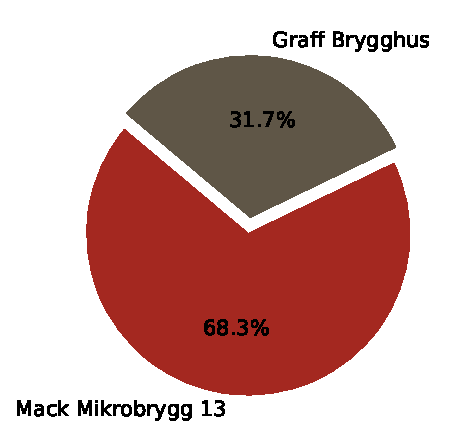
\includegraphics{Kandidatnummer_30_mappeoppgave_2_SOK_2030_files/figure-pdf/cell-41-output-1.pdf}



\end{document}
